% Tài liệu tự học nền tảng cho luận văn tốt nghiệp.
% Biên dịch: latexmk -xelatex location_trajectory_privacy_foundations.tex
\documentclass[11pt,a4paper,oneside]{report}

\usepackage{fontspec}
\setmainfont{Times New Roman}
\setsansfont{Arial}
\usepackage[margin=2.15cm,top=2.25cm,bottom=2.25cm]{geometry}
\usepackage{amsmath,amssymb,mathtools}
\usepackage{microtype}
\usepackage{graphicx}
\usepackage{booktabs,longtable,tabularx,array}
\usepackage{ragged2e}
\usepackage{xcolor}
\usepackage{tikz}
\usetikzlibrary{arrows.meta,positioning,fit,calc,shapes.geometric,backgrounds,decorations.pathreplacing}
\usepackage{caption}
\usepackage[numbers,sort&compress]{natbib}
\usepackage{setspace}
\usepackage{fancyhdr}
\usepackage[hidelinks,unicode]{hyperref}

\definecolor{navy}{HTML}{173B57}
\definecolor{blue}{HTML}{2979A8}
\definecolor{lightblue}{HTML}{EAF4FA}
\definecolor{green}{HTML}{277A5A}
\definecolor{lightgreen}{HTML}{EAF6F0}
\definecolor{red}{HTML}{A33A3A}
\definecolor{lightred}{HTML}{FCEEEE}
\definecolor{amber}{HTML}{A96F12}
\definecolor{lightamber}{HTML}{FFF5DF}
\definecolor{purple}{HTML}{7253A3}
\definecolor{lightpurple}{HTML}{F2EDFA}
\definecolor{graytext}{HTML}{4A545D}
\definecolor{lightgray}{HTML}{F3F5F6}

\hypersetup{
  pdftitle={Nền tảng bảo vệ riêng tư vị trí và quỹ đạo},
  pdfauthor={Ngô Minh Hạnh},
  pdfsubject={Tài liệu tự học dựa trên các công trình của Chow, Mokbel và các nguồn gốc liên quan}
}

\onehalfspacing
\setlength{\parskip}{3pt}
\setlength{\parindent}{1.1cm}
\setlength{\emergencystretch}{2em}
\setlength{\headheight}{14pt}
\captionsetup{font=small,labelfont=bf}

\renewcommand{\chaptername}{Chương}
\renewcommand{\contentsname}{Mục lục}
\renewcommand{\listfigurename}{Danh sách hình}
\renewcommand{\listtablename}{Danh sách bảng}
\renewcommand{\bibname}{Tài liệu tham khảo}
\renewcommand{\figurename}{Hình}
\renewcommand{\tablename}{Bảng}

\pagestyle{fancy}
\fancyhf{}
\fancyhead[L]{\small\sffamily Nền tảng riêng tư vị trí và quỹ đạo}
\fancyhead[R]{\small\sffamily Chow--Mokbel và liên hệ luận văn}
\fancyfoot[C]{\thepage}

\newcolumntype{Y}{>{\RaggedRight\arraybackslash}X}
\newcolumntype{P}[1]{>{\RaggedRight\arraybackslash}p{#1}}
\newcommand{\eng}[1]{\textit{#1}}
\newcommand{\code}[1]{\texttt{#1}}
\newcommand{\truth}{\textcolor{red}{\textbf{dữ liệu thật}}}
\newcommand{\publicout}{\textcolor{blue}{\textbf{đầu ra công khai}}}
\newcommand{\sideinfo}{\textcolor{amber}{\textbf{ngữ cảnh phụ}}}
\newcommand{\attacker}{\textcolor{purple}{\textbf{kẻ tấn công}}}

% Lightweight colored study boxes, kept dependency-free for TeX Live Basic.
\newsavebox{\takeawaystore}
\newsavebox{\definitionstore}
\newsavebox{\warningstore}
\newsavebox{\sourcestore}
\newsavebox{\thesisstore}
\newsavebox{\exercisestore}
\newenvironment{takeaway}[1][Điều cần nhớ]{%
  \par\medskip\noindent\begin{lrbox}{\takeawaystore}\begin{minipage}{.89\textwidth}
  {\sffamily\bfseries\color{blue}#1}\par\smallskip}{%
  \end{minipage}\end{lrbox}\begin{center}\setlength{\fboxsep}{7pt}%
  \fcolorbox{blue}{lightblue}{\usebox{\takeawaystore}}\end{center}\medskip}
\newenvironment{definitionbox}[1][Định nghĩa]{%
  \par\medskip\noindent\begin{lrbox}{\definitionstore}\begin{minipage}{.89\textwidth}
  {\sffamily\bfseries\color{green}#1}\par\smallskip}{%
  \end{minipage}\end{lrbox}\begin{center}\setlength{\fboxsep}{7pt}%
  \fcolorbox{green}{lightgreen}{\usebox{\definitionstore}}\end{center}\medskip}
\newenvironment{warningbox}[1][Cẩn thận]{%
  \par\medskip\noindent\begin{lrbox}{\warningstore}\begin{minipage}{.89\textwidth}
  {\sffamily\bfseries\color{red}#1}\par\smallskip}{%
  \end{minipage}\end{lrbox}\begin{center}\setlength{\fboxsep}{7pt}%
  \fcolorbox{red}{lightred}{\usebox{\warningstore}}\end{center}\medskip}
\newenvironment{sourcebox}[1][Dấu vết nguồn]{%
  \par\medskip\noindent\begin{lrbox}{\sourcestore}\begin{minipage}{.89\textwidth}
  {\sffamily\bfseries\color{graytext}#1}\par\smallskip}{%
  \end{minipage}\end{lrbox}\begin{center}\setlength{\fboxsep}{7pt}%
  \fcolorbox{graytext}{lightgray}{\usebox{\sourcestore}}\end{center}\medskip}
\newenvironment{thesisbox}[1][Nối với luận văn hiện tại]{%
  \par\medskip\noindent\begin{lrbox}{\thesisstore}\begin{minipage}{.89\textwidth}
  {\sffamily\bfseries\color{purple}#1}\par\smallskip}{%
  \end{minipage}\end{lrbox}\begin{center}\setlength{\fboxsep}{7pt}%
  \fcolorbox{purple}{lightpurple}{\usebox{\thesisstore}}\end{center}\medskip}
\newenvironment{exercisebox}[1][Tự kiểm tra]{%
  \par\medskip\noindent\begin{lrbox}{\exercisestore}\begin{minipage}{.89\textwidth}
  {\sffamily\bfseries\color{amber}#1}\par\smallskip}{%
  \end{minipage}\end{lrbox}\begin{center}\setlength{\fboxsep}{7pt}%
  \fcolorbox{amber}{lightamber}{\usebox{\exercisestore}}\end{center}\medskip}

\begin{document}
\hypersetup{pageanchor=false}

\begin{titlepage}
\begin{tikzpicture}[remember picture,overlay]
  \fill[navy] (current page.north west) rectangle ([yshift=-9.0cm]current page.north east);
  \fill[blue] ([yshift=-9.0cm]current page.north west) rectangle ([yshift=-9.18cm]current page.north east);
  \foreach \x/\y/\r in {2.0/-2.0/0.12,3.0/-3.1/0.09,4.3/-1.6/0.10,5.2/-4.1/0.12,6.7/-2.6/0.09,8.1/-4.6/0.11,9.3/-1.7/0.10,10.4/-3.3/0.10,12.2/-2.2/0.12,13.4/-4.3/0.09,15.0/-1.8/0.10,16.7/-3.8/0.12,18.0/-2.5/0.09}{
    \fill[white,opacity=.78] ([xshift=\x cm,yshift=\y cm]current page.north west) circle (\r cm);
  }
  \draw[white,opacity=.43,line width=1.1pt,rounded corners=5pt]
    ([xshift=2cm,yshift=-5.2cm]current page.north west)
    .. controls +(.8,.7) and +(-.7,-.2) .. ([xshift=5.2cm,yshift=-4.1cm]current page.north west)
    .. controls +(.7,.2) and +(-.7,.4) .. ([xshift=8.1cm,yshift=-4.6cm]current page.north west)
    .. controls +(.7,-.2) and +(-.9,-.1) .. ([xshift=13.4cm,yshift=-4.3cm]current page.north west)
    .. controls +(.8,.1) and +(-.7,-.5) .. ([xshift=18cm,yshift=-2.5cm]current page.north west);
\end{tikzpicture}

\vspace*{0.9cm}
{\color{white}\sffamily\Large TÀI LIỆU TỰ HỌC VÀ KIỂM CHỨNG LUẬN VĂN\par}
\vspace{1.0cm}
{\color{white}\sffamily\bfseries\fontsize{24}{30}\selectfont
NỀN TẢNG BẢO VỆ\par
RIÊNG TƯ VỊ TRÍ VÀ QUỸ ĐẠO\par}
\vspace{0.6cm}
{\color{white}\sffamily\Large Từ $k$-anonymity, spatial cloaking và Casper\
đến dummy trajectories và Geo-Indistinguishability\par}

\vspace{3.1cm}
\begin{flushleft}
{\sffamily\Large\bfseries Mục tiêu}\par
\vspace{2mm}
Tái dựng kiến thức nền theo đúng ranh giới giữa \textbf{khái niệm riêng tư},
\textbf{cơ chế}, \textbf{kiến trúc hệ thống}, \textbf{mô hình đối thủ} và
\textbf{metric đánh giá}. Trọng tâm nguồn là survey của Chow--Mokbel và các
công trình gốc về Casper, truy vấn liên tục và dummy trajectories.
\end{flushleft}

\vfill
\noindent\begin{tabularx}{\textwidth}{@{}P{3.6cm}Y@{}}
\textbf{Người học} & Ngô Minh Hạnh\\
\textbf{Đề tài liên hệ} & Bảo vệ tính riêng tư về quỹ đạo cho người dùng dịch vụ dựa trên vị trí\\
\textbf{Phiên bản} & Ngày 03 tháng 09 năm 2026\\
\end{tabularx}
\end{titlepage}

\hypersetup{pageanchor=true}
\pagenumbering{roman}

\chapter*{Cách sử dụng tài liệu}
\addcontentsline{toc}{chapter}{Cách sử dụng tài liệu}

Đừng học các tên thuật toán như một danh sách. Với mỗi phương pháp, hãy tự trả lời
sáu câu hỏi sau:

\begin{enumerate}
  \item \textbf{Bí mật} cần bảo vệ là gì: danh tính, vị trí, toàn quỹ đạo hay nội dung truy vấn?
  \item LSP và đối thủ thật sự \textbf{nhìn thấy đầu ra nào}?
  \item Thành phần nào được \textbf{tin cậy} và thành phần nào không?
  \item Đối thủ có \textbf{ngữ cảnh phụ} gì: bản đồ, tốc độ, POI, lịch sử, prior dân số?
  \item Cơ chế hứa một \textbf{bảo đảm} toán học hay chỉ một mục tiêu thiết kế?
  \item Metric có thật sự đo đúng lời hứa đó hay không?
\end{enumerate}

Mỗi chương đi theo nhịp \emph{định nghĩa $\rightarrow$ ví dụ $\rightarrow$ giả định
$\rightarrow$ cách thất bại $\rightarrow$ liên hệ luận văn}. Các hình trong tài liệu
đều là sơ đồ tự dựng từ khái niệm của nguồn được trích dẫn; không sao chép hình
nguyên bản trong paper.

\begin{warningbox}[Một chỉnh sửa nguồn ngay từ đầu]
Internship 2 chỉ dẫn trực tiếp \textbf{một} công trình có đồng tác giả Mohamed F.
Mokbel: survey Chow--Mokbel năm 2011. Metadata ở bibliography cũ ghi nhầm venue
và trang; bản đúng là \emph{ACM SIGKDD Explorations}, tập 13 số 1, trang 19--29,
DOI \href{https://doi.org/10.1145/2031331.2031335}{10.1145/2031331.2031335}
\cite{chow2011trajectory}. Tài liệu này bổ sung các paper gốc Casper và dummy để
không gán nhầm mọi ý tưởng cho survey.
\end{warningbox}

\tableofcontents
\listoffigures
\listoftables

\clearpage
\chapter*{Bản đồ một trang}
\addcontentsline{toc}{chapter}{Bản đồ một trang}

\begin{figure}[htbp]
\centering
\resizebox{\textwidth}{!}{%
\begin{tikzpicture}[
  font=\small\sffamily,
  node distance=9mm and 12mm,
  q/.style={draw=navy,fill=lightblue,rounded corners,minimum width=36mm,minimum height=13mm,align=center},
  a/.style={draw=amber,fill=lightamber,rounded corners,minimum width=42mm,minimum height=13mm,align=center},
  p/.style={draw=purple,fill=lightpurple,rounded corners,minimum width=42mm,minimum height=13mm,align=center},
  arr/.style={-{Latex[length=2mm]},line width=.8pt,draw=graytext}
]
\node[q] (secret) {1. Bí mật\\$x_t,\ T,\ id,\ q_t$};
\node[q,right=of secret] (criterion) {2. Tiêu chí/bảo đảm\\$k$-anonymity, Geo-I};
\node[q,right=of criterion] (mechanism) {3. Cơ chế\\cloaking, dummy, noise};
\node[q,right=of mechanism] (system) {4. Kiến trúc\\Casper, P2P, on-device};
\node[a,below=of criterion] (context) {5. Đối thủ + ngữ cảnh\\map, time, POI, history, prior};
\node[p,below=of mechanism] (metric) {6. Bằng chứng\\formal proof + attack + utility};
\draw[arr] (secret)--(criterion);
\draw[arr] (criterion)--(mechanism);
\draw[arr] (mechanism)--(system);
\draw[arr] (system.south) |- (metric.east);
\draw[arr] (context)--(metric);
\draw[arr] (mechanism)--(metric);
\draw[arr] (secret.south) |- (context.west);
\end{tikzpicture}}
\caption{Sáu lớp phải tách riêng khi đọc một phương pháp bảo vệ riêng tư.}
\label{fig:six-layers}
\end{figure}

\begin{table}[htbp]
\centering
\small
\caption{Các thuật ngữ thường bị dùng lẫn, nhưng bản chất khác nhau.}
\label{tab:concept-map}
\begin{tabularx}{\textwidth}{P{3.2cm}P{3.4cm}Y}
\toprule
\textbf{Thuật ngữ} & \textbf{Nó là gì?} & \textbf{Câu hỏi mà nó trả lời} \\
\midrule
$k$-anonymity & Tiêu chí ẩn danh & Bản ghi/người dùng có hòa vào nhóm ít nhất $k$ đối tượng không?\\
Spatial cloaking & Cơ chế biến điểm thành vùng & Thay vì gửi tọa độ thật, ta gửi vùng nào?\\
Casper & Kiến trúc hệ thống & Ai cloak, LSP xử lý vùng ra sao, ai lọc candidate?\\
Dummy generation & Chiến lược tạo đầu ra giả & Gửi thêm hoặc thay thế bằng những điểm/quỹ đạo giả nào?\\
Geo-I & Bảo đảm xác suất theo khoảng cách & Hai vị trí thật gần nhau tạo phân phối đầu ra giống nhau đến đâu?\\
Attacker model & Bài toán suy luận & Đối thủ quan sát gì, biết gì và tối ưu mục tiêu nào?\\
Metric & Phép đo bằng chứng & Kết quả nào chứng minh privacy/utility/overhead?\\
\bottomrule
\end{tabularx}
\end{table}

\begin{takeaway}
\textbf{Câu neo trí nhớ:} $k$-anonymity không phải một generator; cloaking không
phải toàn bộ Casper; Casper không sinh dummy; có $K$ dummy không tự động tạo
$k$-anonymity; Geo-I không tự động bảo đảm một quỹ đạo hợp lý.
\end{takeaway}

\clearpage
\pagenumbering{arabic}

% ============================================================================
\chapter{Vẽ đúng bài toán trước khi chọn thuật toán}

\section{Một lần dùng LBS chứa nhiều hơn một tọa độ}

Một sự kiện dịch vụ dựa trên vị trí (LBS) ở thời điểm $t$ có thể mô hình hóa là
\[
e_t=(u,\,s,\,x_t,\,t,\,q_t),
\]
trong đó $u$ là định danh hoặc pseudonym, $s$ là phiên, $x_t$ là vị trí, $t$ là
thời gian và $q_t$ là nội dung truy vấn. Một transcript liên tục là
$O_{1:T}=(o_1,\ldots,o_T)$, tức toàn bộ những gì phía không tin cậy quan sát sau
khi cơ chế bảo vệ đã chạy.

\begin{definitionbox}[Điểm, mẫu, quỹ đạo và transcript]
\begin{itemize}
  \item \textbf{Điểm vị trí} $x_t=(lat_t,lon_t)$ chỉ nói ``ở đâu'' tại một thời điểm.
  \item \textbf{Mẫu không gian--thời gian} $p_t=(x_t,t)$ còn cho biết ``khi nào''.
  \item \textbf{Quỹ đạo} $T=(p_1,\ldots,p_T)$ nối các mẫu có thứ tự; trên mạng đường,
  các điểm còn bị ràng buộc bởi cạnh, hướng và thời gian đi.
  \item \textbf{Transcript} có thể chứa pseudonym, batch dummy, truy vấn, kết quả,
  thời lượng phiên và metadata. Đây mới là đầu vào thực tế của attacker.
\end{itemize}
\end{definitionbox}

Một pseudonym chỉ xóa tên trực tiếp. Chuỗi ``rời một căn nhà lúc 7:30, đến một cơ
quan lúc 8:15, ghé phòng khám vào thứ Ba'' vẫn có thể đóng vai trò
\eng{quasi-identifier}. Chow--Mokbel nhấn mạnh rằng tương quan không gian và thời
gian làm bài toán quỹ đạo khó hơn bảo vệ một snapshot độc lập
\cite{chow2011trajectory}.

\begin{figure}[htbp]
\centering
\begin{tikzpicture}[
  font=\small\sffamily,
  box/.style={draw=navy,fill=lightblue,rounded corners,minimum width=34mm,minimum height=14mm,align=center},
  sem/.style={draw=amber,fill=lightamber,rounded corners,minimum width=36mm,minimum height=14mm,align=center},
  arr/.style={-{Latex[length=2mm]},thick,draw=blue},
  node distance=8mm
]
\node[box] (x) {tọa độ\\$x_t$};
\node[box,right=of x] (p) {mẫu\\$(x_t,t)$};
\node[box,right=of p] (tr) {chuỗi\\$T=(p_1,\ldots,p_T)$};
\node[sem,right=of tr] (meaning) {ngữ nghĩa\\nhà $\rightarrow$ nơi làm\\$\rightarrow$ phòng khám};
\draw[arr] (x)-- node[above,font=\scriptsize]{thêm thời gian} (p);
\draw[arr] (p)-- node[above,font=\scriptsize]{liên kết} (tr);
\draw[arr] (tr)-- node[above,font=\scriptsize]{ghép POI/lịch sử} (meaning);
\end{tikzpicture}
\caption{Thông tin nhạy cảm tăng khi một điểm được liên kết theo thời gian và gắn ngữ nghĩa.}
\label{fig:data-evolution}
\end{figure}

\section{Hai trục phân biệt quyết định toàn bộ thiết kế}

\subsection{Snapshot và continuous LBS}

\textbf{Snapshot LBS} xử lý một lần hỏi tại một thời điểm, chẳng hạn ``quán cà phê
gần tôi nhất''. \textbf{Continuous LBS} duy trì truy vấn qua nhiều lần cập nhật,
chẳng hạn ``liên tục báo trạm xăng gần nhất khi tôi đang lái xe''. Ở snapshot,
attacker lọc candidate trong một khung hình; ở continuous, attacker còn nối các
khung hình bằng vận tốc, hướng đi và lịch sử.

\subsection{Dùng dịch vụ trực tuyến và công bố dataset ngoại tuyến}

\begin{table}[htbp]
\centering
\small
\caption{Hai bài toán cùng dùng từ ``trajectory privacy'' nhưng không thể đánh đồng.}
\label{tab:online-offline}
\begin{tabularx}{\textwidth}{P{3.4cm}Y Y}
\toprule
 & \textbf{Continuous LBS trực tuyến} & \textbf{Trajectory publication ngoại tuyến}\\
\midrule
Mục đích & Nhận dịch vụ ngay khi đang di chuyển & Phát hành dataset cho phân tích/mining\\
Dữ liệu sẵn có & Tương lai chưa biết; update tốc độ cao & Có thể nhìn toàn bộ dataset tĩnh\\
Ràng buộc & Độ trễ, băng thông, giao thức query & Chất lượng thống kê sau biến đổi\\
Cơ chế điển hình & Cloaking, mix-zone, path confusion, dummy & Clustering, generalization, suppression\\
Đầu ra & Request/transcript tác nghiệp & Dataset đã ẩn danh/tổng hợp\\
\bottomrule
\end{tabularx}
\end{table}

Survey Chow--Mokbel tách rõ hai nhánh này: giải pháp online phải xử lý update động
và chưa biết chuyển động tương lai, còn publication có thể tối ưu toàn cục trên dữ
liệu hoàn chỉnh \cite{chow2011trajectory}. Một generator phục vụ query online
không nên được đánh giá như một mô hình sinh synthetic dataset, và ngược lại.

\section{Bốn bí mật khác nhau}

\begin{table}[htbp]
\centering
\small
\caption{Bốn mục tiêu bảo vệ cần được phát biểu thành bốn nhiệm vụ suy luận riêng.}
\label{tab:privacy-targets}
\begin{tabularx}{\textwidth}{P{3.0cm}Y Y}
\toprule
\textbf{Mục tiêu} & \textbf{Câu hỏi của attacker} & \textbf{Ví dụ bằng chứng}\\
\midrule
Danh tính & Transcript này thuộc về ai? & Accuracy tái định danh; linkability\\
Vị trí & Người dùng thật ở đâu tại $t$? & Sai số suy luận; xác suất trong bán kính $r$\\
Quỹ đạo/đường kế tiếp & Chuỗi thật hoặc cạnh tiếp theo là gì? & DTW/Hausdorff, next-edge accuracy\\
Nội dung truy vấn & Người dùng đang tìm loại POI/dịch vụ nào? & Query-class accuracy; semantic leakage\\
\bottomrule
\end{tabularx}
\end{table}

\begin{warningbox}
Một cơ chế có thể giấu vị trí nhưng vẫn để lộ nội dung truy vấn; hoặc làm đường đi
khó tái dựng nhưng vẫn bị link về đúng người dùng. Không được dùng một metric duy
nhất rồi kết luận cả bốn mục tiêu đều an toàn.
\end{warningbox}

\section{Khung sáu biến để đọc mọi paper}

Ta ký hiệu một cơ chế $M$ nhận bí mật $X$, ngữ cảnh công khai $C_{pub}$ và randomness
$R$, rồi tạo quan sát $O=M(X,C_{pub};R)$. Đối thủ có thêm side information $C_A$
và suy luận
\[
\Pr(X\mid O,C_A)\propto \Pr(O\mid X,C_A)\Pr(X\mid C_A).
\]
Mọi claim privacy đều phụ thuộc ít nhất vào: miền bí mật $X$, đầu ra $O$, trust
boundary, kiến thức $C_A$, bảo đảm của $M$ và thước đo trên posterior/utility.

\begin{exercisebox}
Ứng dụng gửi 5 vị trí cùng một pseudonym qua 20 lần cập nhật. Hãy viết rõ: (i) secret
là gì; (ii) LSP thấy gì; (iii) attacker có thể dùng side information nào. Nếu chỉ nói
``có $k=5$ nên xác suất đúng là $1/5$'', ta đã bỏ qua biến nào trong công thức Bayes?
\end{exercisebox}

% ============================================================================
\chapter{\texorpdfstring{$k$}{k}-anonymity và spatial cloaking}

\section{\texorpdfstring{$k$}{k}-anonymity nguyên thủy: ẩn trong một lớp tương đương}

$k$-anonymity xuất phát từ bài toán phát hành bảng dữ liệu, với nền tảng của
Samarati và Sweeney \cite{samarati2001,sweeney2002}. Một tập thuộc tính như tuổi,
mã vùng và giới tính có thể không phải tên trực tiếp nhưng vẫn liên kết được với
nguồn ngoài; chúng là \eng{quasi-identifiers}.

\begin{definitionbox}[$k$-anonymity trong bảng dữ liệu]
Một bảng đạt $k$-anonymity đối với tập quasi-identifier $Q$ nếu mỗi tổ hợp giá trị
công khai trên $Q$ xuất hiện trong ít nhất $k$ bản ghi. Các bản ghi có cùng giá trị
trên $Q$ tạo thành một \textbf{lớp tương đương}.
\end{definitionbox}

Ví dụ, sau khi tổng quát hóa tuổi thành 20--29 và mã vùng thành 700**, nếu bốn bản
ghi giống nhau trên hai cột đó thì mỗi người hòa vào một lớp tương đương có kích
thước 4. Tuy nhiên, nếu cả bốn đều có cùng bệnh nhạy cảm thì thuộc tính nhạy cảm
vẫn lộ. Đây là lý do $k$-anonymity không giải quyết mọi dạng background knowledge.

\section{Chuyển sang LBS: ẩn trong một vùng có người thật}

Spatial cloaking thay điểm thật $x_t$ bằng một vùng $R_t$. Một cách diễn giải phổ
biến là
\[
|U(R_t)|\ge k,
\qquad
\operatorname{area}(R_t)\ge A_{\min},
\]
trong đó $U(R_t)$ là tập \textbf{người dùng thật} nằm trong vùng. The New Casper
dùng profile cốt lõi $(k,A_{\min})$; bản Casper* sau đó mô tả thêm $A_{\max}$ như
giới hạn bất chính xác lớn nhất mà người dùng chấp nhận
\cite{mokbel2006casper,chow2009casper}.

\begin{figure}[htbp]
\centering
\resizebox{0.96\textwidth}{!}{%
\begin{tikzpicture}[font=\small\sffamily]
  % dense panel
  \begin{scope}[xshift=0cm]
    \draw[step=.7cm,gray!25,very thin] (0,0) grid (6.3,4.9);
    \node[anchor=south west,font=\bfseries] at (0,5.05) {Khu đông người};
    \foreach \x/\y/\n in {2.2/2.2/A,2.6/2.5/B,3.0/2.0/C,2.9/2.8/D,4.8/1.2/E,1.1/4.0/F}{
      \fill[blue] (\x,\y) circle (2.6pt); \node[above right=-1pt,font=\scriptsize] at (\x,\y) {\n};}
    \draw[red,very thick,rounded corners] (2.0,1.8) rectangle (3.25,3.05);
    \node[red,font=\bfseries] at (2.65,1.55) {$k=4$};
    \draw[amber,dashed,very thick,rounded corners] (1.55,1.35) rectangle (3.75,3.55);
    \node[amber,font=\bfseries] at (3.15,3.78) {$A_{\min}$};
  \end{scope}
  % sparse panel
  \begin{scope}[xshift=8cm]
    \draw[step=.7cm,gray!25,very thin] (0,0) grid (6.3,4.9);
    \node[anchor=south west,font=\bfseries] at (0,5.05) {Khu thưa người};
    \foreach \x/\y/\n in {1.0/2.3/A,2.6/3.6/B,4.9/3.0/C,5.5/.9/D,1.5/.6/E}{
      \fill[blue] (\x,\y) circle (2.6pt); \node[above right=-1pt,font=\scriptsize] at (\x,\y) {\n};}
    \draw[red,very thick,rounded corners] (.65,.55) rectangle (5.15,3.9);
    \node[red,font=\bfseries] at (3.0,4.15) {vùng cần lớn để đủ $k=4$};
  \end{scope}
\end{tikzpicture}}
\caption{Sơ đồ tự dựng: cùng $k=4$, vùng ở nơi đông có thể quá nhỏ; $A_{\min}$ đặt thêm ngưỡng không gian. Ở nơi thưa, vùng phải mở rộng nhiều và làm tăng chi phí query.}
\label{fig:k-area}
\end{figure}

\subsection{Tại sao cần cả \texorpdfstring{$k$}{k} và \texorpdfstring{$A_{\min}$}{A-min}?}

Trong sân vận động, 100 người có thể đứng trong một vùng rất nhỏ: $k=100$ nhưng
độ chính xác không gian vẫn cao. $A_{\min}$ ngăn vùng bị nhỏ hơn mức người dùng
chấp nhận. Ngược lại, ở khu thưa người, việc tìm đủ $k$ người có thể tạo vùng rất
lớn; $A_{\max}$ trong profile mở rộng có thể giới hạn mức suy giảm utility. Privacy
profile vì vậy mô tả một trade-off, không phải ``càng tăng mọi tham số càng tốt''
\cite{chow2009casper}.

\section{\texorpdfstring{$k$}{k} không tự động cho posterior \texorpdfstring{$1/k$}{1/k}}

Giả sử một vùng chứa bốn người $A,B,C,D$. Nếu attacker không có cách phân biệt
và prior cân bằng, posterior có thể là $(0.25,0.25,0.25,0.25)$. Nhưng khi biết người
gửi thường đến bệnh viện vào thứ Ba, posterior có thể thành
\[
(0.70,0.10,0.10,0.10).
\]
Vùng vẫn chứa bốn người, nhưng chiến lược đoán tốt nhất đúng với xác suất 0.70,
không phải 0.25. Chow--Mokbel cũng cảnh báo rằng semantic/background information
có thể làm đối thủ suy ra vị trí với độ chắc chắn cao hơn
\cite{chow2011trajectory}.

\begin{warningbox}[Ba câu không được viết trong luận văn nếu thiếu điều kiện]
\begin{itemize}
  \item ``Có $k$ candidate nên xác suất đoán đúng bằng $1/k$.''
  \item ``$k$ càng lớn thì privacy chắc chắn càng cao.''
  \item ``Có $K$ dummy nghĩa là cơ chế đạt $k$-anonymity.''
\end{itemize}
Các câu này chỉ gần đúng khi candidate thật sự không phân biệt được dưới mô hình
đối thủ đã phát biểu. $k$-anonymity dựa trên \textbf{người thật trong vùng} còn
dummy set dựa trên \textbf{đầu ra do một client tạo}; hai khái niệm không đồng nhất.
\end{warningbox}

\section{Ba kiến trúc spatial cloaking}

\begin{figure}[htbp]
\centering
\resizebox{\textwidth}{!}{%
\begin{tikzpicture}[
 font=\scriptsize\sffamily,
 dev/.style={draw=green,fill=lightgreen,rounded corners,minimum width=24mm,minimum height=10mm,align=center},
 mid/.style={draw=navy,fill=lightblue,rounded corners,minimum width=30mm,minimum height=12mm,align=center},
 lsp/.style={draw=red,fill=lightred,rounded corners,minimum width=28mm,minimum height=12mm,align=center},
 arr/.style={-{Latex[length=1.8mm]},thick,draw=graytext}
]
\node[font=\small\bfseries] at (2.6,3.8) {Tập trung/Casper};
\node[dev] (u1) at (0.8,2.6) {người dùng\\vị trí thật};
\node[mid] (an) at (3.0,2.6) {trusted\\anonymizer};
\node[lsp] (s1) at (5.5,2.6) {LSP\\vùng cloaked};
\draw[arr] (u1)--(an); \draw[arr] (an)--(s1);

\node[font=\small\bfseries] at (9.2,3.8) {Phân tán qua hạ tầng};
\node[dev] (u2) at (7.0,2.6) {client A};
\node[mid] (ds) at (9.2,2.6) {cấu trúc chia sẻ\\/base station};
\node[lsp] (s2) at (11.7,2.6) {LSP};
\draw[arr] (u2)--(ds); \draw[arr] (ds)--(s2);

\node[font=\small\bfseries] at (15.6,3.8) {Peer-to-peer};
\node[dev] (p1) at (13.5,2.9) {peer A};
\node[dev] (p2) at (15.4,1.7) {peer B};
\node[dev] (p3) at (15.7,3.0) {peer C};
\node[lsp] (s3) at (18.1,2.6) {LSP};
\draw[arr] (p1)--(p2); \draw[arr] (p2)--(p3); \draw[arr] (p3)--(s3);
\end{tikzpicture}}
\caption{Ba họ kiến trúc cloaking. P2P bỏ điểm trung gian tập trung nhưng thêm bài toán khám phá peer, mobility, partition và chia sẻ vị trí giữa các peer.}
\label{fig:cloaking-architectures}
\end{figure}

Trong kiến trúc tập trung, anonymizer biết vị trí thật và trở thành điểm tin cậy lẫn
điểm lỗi tập trung. Mô hình phân tán duy trì cấu trúc thông tin qua hạ tầng. Mô hình
P2P để các thiết bị phối hợp trực tiếp; Chow, Mokbel và Liu bổ sung cơ chế chia sẻ
thông tin, dùng vị trí lịch sử khi network partition và điều chỉnh vùng để tránh
\eng{center-of-cloaked-area attack} \cite{chow2011p2p}.

Mô hình P2P đó giả định các peer được tin cậy khi trao đổi vị trí và chỉ xử lý
snapshot queries. Xác suất $1/K$ của bước điều chỉnh tâm thuộc đúng center estimator
với vị trí peer chính xác; khi chỉ có vị trí lịch sử/bất định, cơ chế chủ yếu làm giảm
rủi ro chứ không tạo một posterior guarantee phổ quát.

\section{Cloaking trên mạng đường}

Một hình chữ nhật Euclid có thể chứa nhiều diện tích không thể đi được (sông, tòa
nhà) nhưng chỉ cắt đúng một đoạn đường. Vì vậy ``diện tích lớn'' không đồng nghĩa
``nhiều vị trí đường đi khả dĩ''. Query-aware location anonymization của Chow,
Mokbel, Bao và Liu biểu diễn output bằng các đoạn đường liên thông, yêu cầu ít nhất
$K$ người và tổng chiều dài đường tối thiểu $L$, đồng thời cân bằng kích thước
candidate target list với ước lượng chi phí thực thi query
\cite{chow2011road}.

\begin{figure}[htbp]
\centering
\begin{tikzpicture}[font=\small\sffamily]
  \fill[blue!8] (0,0) rectangle (6,4);
  \draw[blue,very thick] (0,0) rectangle (6,4);
  \draw[gray!60,line width=3pt] (-.5,2)--(6.5,2);
  \fill[red] (3.1,2) circle (3pt);
  \node[red,below] at (3.1,1.8) {một đoạn khả dĩ};
  \node[blue,font=\bfseries] at (3,4.35) {vùng Euclid lớn};
  \draw[gray!60,line width=3pt] (8,1)--(10,1)--(12,2.6)--(15,2.6);
  \draw[gray!60,line width=3pt] (10,.2)--(10,3.8);
  \draw[gray!60,line width=3pt] (12,.2)--(12,3.8);
  \draw[green,very thick] (8.8,1)--(10,1)--(12,2.6)--(13.7,2.6);
  \foreach \x/\y in {9.2/1,10/1.7,12/2.6,13.2/2.6}{\fill[blue] (\x,\y) circle (2.7pt);}
  \node[green,font=\bfseries,align=center] at (11.5,4.35) {road cloak: đoạn liên thông\\$K$ users + độ dài $L$};
\end{tikzpicture}
\caption{Sơ đồ tự dựng: metric diện tích Euclid và metric chiều dài/khả đạt trên road graph trả lời hai câu hỏi khác nhau.}
\label{fig:road-cloak}
\end{figure}

Đây vẫn là \textbf{road-segment cloaking}, không phải dummy trajectory hay Geo-I.
``Query-aware quality'' trong paper là kích thước candidate target list và chi phí
thực thi trên road network;
không nên đồng nhất với POI recall/NDCG của thesis hiện tại.

\begin{exercisebox}
Một khu có 12 người đứng rất sát nhau trong cửa hàng. Với $k=10$, vùng cloak chỉ
rộng 20 m$^2$. Hãy giải thích vì sao vẫn có thể cần $A_{\min}=10{,}000$ m$^2$, và
việc đó sẽ tác động thế nào tới candidate answers của truy vấn ``nearest hospital''.
\end{exercisebox}

% ============================================================================
\chapter{Casper: cloaking chỉ là nửa đầu của hệ thống}

\section{Bài toán ``tìm bệnh viện gần nhất''}

Nếu chỉ gửi một hình chữ nhật thay cho điểm thật, database không còn biết chính
xác vị trí nào trong vùng là vị trí truy vấn. Vì vậy hệ thống cần hai phần ghép
khớp với nhau:

\begin{enumerate}
  \item \textbf{Location anonymizer} biến vị trí thật thành vùng thỏa privacy profile.
  \item \textbf{Privacy-aware query processor} xử lý trực tiếp vùng đó và trả về một
  tập candidate chắc chắn chứa đáp án cần thiết.
\end{enumerate}

Đây là tư tưởng trung tâm của The New Casper và bản mở rộng Casper*
\cite{mokbel2006casper,chow2009casper}. Casper* độc lập với thuật toán tạo vùng cụ
thể, miễn vùng đầu vào là rectilinear cloaked area mà query processor hiểu được.

\begin{figure}[htbp]
\centering
\resizebox{0.98\textwidth}{!}{%
\begin{tikzpicture}[
  font=\small\sffamily,
  node distance=8mm and 8mm,
  trusted/.style={draw=green,fill=lightgreen,rounded corners,minimum width=34mm,minimum height=15mm,align=center},
  untrusted/.style={draw=red,fill=lightred,rounded corners,minimum width=38mm,minimum height=15mm,align=center},
  output/.style={draw=blue,fill=lightblue,rounded corners,minimum width=35mm,minimum height=15mm,align=center},
  arr/.style={-{Latex[length=2mm]},thick,draw=graytext}
]
\node[trusted] (phone) {1. Thiết bị\\$x$, query, $(k,A_{\min})$};
\node[trusted,right=of phone] (anon) {2. Anonymizer\\$x\mapsto R$; bỏ định danh};
\node[untrusted,right=of anon] (lsp) {3. LSP\\query processor trên vùng};
\node[output,right=of lsp] (cand) {4. Candidate list\\$C(R)$};
\node[trusted,below=12mm of anon] (refine) {5. Refine với $x$\\đáp án chính xác};
\draw[arr] (phone)-- node[above,font=\scriptsize]{vị trí thật} (anon);
\draw[arr] (anon)-- node[above,font=\scriptsize]{vùng $R$} (lsp);
\draw[arr] (lsp)--(cand);
\draw[arr] (cand.south) |- (refine.east);
\draw[arr] (refine.west) -| (phone.south);
\begin{scope}[on background layer]
  \node[draw=green,dashed,rounded corners,fit=(phone)(anon)(refine),inner sep=4mm,
    label={[font=\scriptsize\sffamily,text=green]below:vùng tin cậy}] {};
\end{scope}
\end{tikzpicture}}
\caption{Pipeline Casper được vẽ lại: LSP không thấy điểm thật nhưng phải trả một superset đủ để phía tin cậy tinh chỉnh thành đáp án đúng.}
\label{fig:casper-pipeline}
\end{figure}

\begin{takeaway}
\textbf{Casper không tạo dummy.} Nó dựa vào quần thể người dùng thật để tạo vùng
$k$-anonymous, cần một anonymizer tin cậy, và sửa query processor phía server để
bù cho việc mất độ chính xác không gian.
\end{takeaway}

\section{Anonymizer ``tìm đủ \texorpdfstring{$k$}{k} người'' như thế nào?}

Hãy tưởng tượng bản đồ được chia thành các ô nhỏ và các ô được nhóm thành ô cha
lớn dần. Anonymizer biết vị trí cập nhật của quần thể đang hoạt động:

\begin{enumerate}
  \item bắt đầu ở ô nhỏ chứa người phát query;
  \item đếm \textbf{người thật} trong ô và kiểm tra diện tích;
  \item nếu chưa đủ $k$ hoặc chưa đạt $A_{\min}$, ghép ô lân cận/đi lên ô cha;
  \item dừng khi profile thỏa, bỏ identity rồi phát hành vùng.
\end{enumerate}

The New Casper dùng một grid pyramid và phiên bản adaptive để không phải lưu mọi ô
ở mọi tầng \cite{mokbel2006casper}. Nhiều cloaker khác có thể chọn vùng khác; query
processor của Casper* được thiết kế độc lập với thuật toán cloaking cụ thể, miễn
nhận rectilinear region \cite{chow2009casper}.

\begin{warningbox}
``Tìm $k$'' ở đây không phải random lấy $k$ tọa độ quanh truth. Nó tìm $k$ người
thật đang được anonymizer theo dõi. Nếu hệ thống chỉ có một client tự tạo $K$ điểm,
ta đã chuyển sang dummy generation và không còn đúng semantics này.
\end{warningbox}

\section{Tại sao candidate list giữ được utility?}

Giả sử vị trí thật nằm ở đâu đó trong vùng $R$. Với truy vấn nearest neighbor,
LSP phải trả những đối tượng có thể là gần nhất đối với \emph{ít nhất một} điểm
trong $R$ hoặc một superset an toàn của tập tối thiểu đó. Nếu trả đúng một bệnh
viện gần tâm hình chữ nhật, bệnh viện ấy có thể sai đối với người ở góc xa. Phía
tin cậy dùng $x$ để chọn đáp án chính xác từ candidate list
\cite{chow2009casper}.

\begin{figure}[htbp]
\centering
\begin{tikzpicture}[font=\small\sffamily,scale=.92]
  \draw[gray!35,step=.8cm,very thin] (0,0) grid (10.4,5.6);
  \fill[lightblue,opacity=.8] (3.0,1.6) rectangle (6.8,4.4);
  \draw[blue,very thick] (3.0,1.6) rectangle (6.8,4.4);
  \node[blue,font=\bfseries] at (4.9,4.7) {vùng cloaked $R$};
  \fill[red] (4.1,2.4) circle (3.2pt); \node[red,below right] at (4.1,2.4) {$x$ (ẩn với LSP)};
  \foreach \x/\y/\n in {2.0/3.2/H_1,5.2/5.0/H_2,7.8/3.6/H_3,6.8/.8/H_4,9.2/1.8/H_5}{
    \draw[green,thick] (\x-.13,\y)--(\x+.13,\y); \draw[green,thick] (\x,\y-.13)--(\x,\y+.13);
    \node[green,above right=-1pt] at (\x,\y) {$\n$};}
  \draw[dashed,graytext] (4.1,2.4)--(2.0,3.2);
  \node[draw=green,fill=lightgreen,rounded corners,align=left] at (12.6,3.2)
    {LSP trả $C(R)=\{H_1,H_2,H_3,H_4\}$\\Phía tin cậy biết $x$\\và chọn đúng $H_1$};
  \draw[-{Latex},thick,green] (7.9,3.2)--(10.7,3.2);
\end{tikzpicture}
\caption{Sơ đồ trực giác của query refinement; tập candidate có thể lớn hơn tập tối thiểu để đổi lấy khả năng mở rộng hệ thống.}
\label{fig:casper-candidates}
\end{figure}

Casper* phân loại cả private query trên public data, public query trên private data,
và private query trên private data. Với luận văn hiện tại, trường hợp gần nhất là
private query trên public POI/map; nhưng output contract của luận văn không phải
vùng $R$, nên không thể bê nguyên query processor của Casper sang mà không đổi
giao thức.

\section{Privacy--utility--system cost trong Casper}

Ba đại lượng chuyển động cùng nhau:

\begin{itemize}
  \item Privacy profile nghiêm ngặt hơn thường làm vùng $R$ lớn hơn.
  \item Vùng lớn hơn làm candidate list, I/O, CPU và băng thông tăng.
  \item Query refinement giúp giữ đáp án cuối chính xác, nhưng không làm chi phí biến mất.
\end{itemize}

Do đó ``utility'' trong Casper không chỉ là khoảng cách giữa điểm thật và vùng cloak;
nó còn gồm độ đầy đủ của candidate answer, độ trễ và chi phí truyền. Casper* đưa
các tuning parameter để đổi giữa khả năng mở rộng và tính tối ưu của candidate list
\cite{chow2009casper}.

\section{Ranh giới tin cậy và failure modes}

\begin{center}
\begin{minipage}{\textwidth}
\centering
\small
\captionof{table}{Giả định của Casper và điều xảy ra khi giả định hỏng.}
\label{tab:casper-failures}
\begin{tabularx}{\textwidth}{P{4.2cm}Y Y}
\toprule
\textbf{Giả định} & \textbf{Vai trò} & \textbf{Khi hỏng}\\
\midrule
Anonymizer đáng tin & Nhìn thấy exact location, bỏ identity, refine answer & Trở thành nơi tập trung lịch sử vị trí và điểm tấn công\\
Có đủ người dùng thật & Tạo vùng chứa ít nhất $k$ người & Khu thưa phải chờ/mở rộng hoặc không đáp ứng profile\\
Query processor hiểu vùng & Trả candidate list an toàn & Dịch vụ truyền thống có thể trả kết quả sai hoặc không hỗ trợ\\
Thành viên khó phân biệt & Nối set size với uncertainty & Prior, semantic hoặc mật độ bất đều làm posterior lệch\\
Không lạm dụng chuỗi thời gian & Bảo vệ snapshot & Continuous tracking làm giao tập ứng viên co lại\\
\bottomrule
\end{tabularx}
\end{minipage}
\end{center}

\begin{exercisebox}
Hãy trình bày Casper trong 30 giây mà bắt buộc có đủ bốn từ: \emph{trusted
anonymizer}, \emph{cloaked region}, \emph{candidate list}, \emph{refinement}.
Nếu thiếu một từ, câu chuyện hệ thống đang mất mắt xích nào?
\end{exercisebox}

% ============================================================================
\chapter{Khi snapshot trở thành chuỗi: các tấn công liên tục}

\section{Đủ \texorpdfstring{$k$}{k} ở từng thời điểm vẫn có thể lộ}

Giả sử một continuous query có ba cloaked regions. Mỗi vùng đều chứa bốn người:
\[
S_1=\{A,B,C,D\},\quad
S_2=\{A,B,E,F\},\quad
S_3=\{A,G,H,I\}.
\]
Từng snapshot trông như 4-anonymous. Nhưng nếu LSP biết ba vùng thuộc cùng một
phiên thì
\[
S_1\cap S_2\cap S_3=\{A\}.
\]
Đây là trực giác của \eng{query tracking attack} mà Chow--Mokbel phân tích
\cite{chow2007continuous}.

\begin{figure}[htbp]
\centering
\resizebox{0.95\textwidth}{!}{%
\begin{tikzpicture}[font=\small\sffamily]
\foreach \dx/\label in {0/$t_1$,5.2/$t_2$,10.4/$t_3$}{
  \begin{scope}[xshift=\dx cm]
    \draw[blue,very thick,rounded corners,fill=lightblue] (0,0) rectangle (4.0,3.2);
    \node[font=\bfseries] at (2,3.55) {\label};
  \end{scope}}
\node[font=\bfseries,blue] at (2,.35) {$\{A,B,C,D\}$};
\node[font=\bfseries,blue] at (7.2,.35) {$\{A,B,E,F\}$};
\node[font=\bfseries,blue] at (12.4,.35) {$\{A,G,H,I\}$};
\foreach \dx/\x/\y/\n in {0/.7/2.4/A,0/1.7/1.7/B,0/3.1/2.4/C,0/3.3/1.2/D,
5.2/.8/2.3/A,5.2/1.9/1.6/B,5.2/3.1/2.4/E,5.2/3.3/1.0/F,
10.4/.8/2.2/A,10.4/1.8/1.3/G,10.4/3.0/2.4/H,10.4/3.3/1.0/I}{
  \fill[blue] (\dx+\x,\y) circle (2.7pt);
  \node[above right=-1pt] at (\dx+\x,\y) {\n};}
\draw[red,very thick,-{Latex[length=2mm]}] (.7,2.4) .. controls (4.1,4.2) and (6.0,4.2) .. (6.0,2.3)
  .. controls (9.3,4.0) and (10.2,3.7) .. (11.2,2.2);
\node[red,font=\bfseries] at (7.1,4.45) {chỉ $A$ sống qua cả ba snapshot};
\end{tikzpicture}}
\caption{Intersection/query-tracking attack: set size tại mỗi thời điểm không ngăn liên kết xuyên thời gian.}
\label{fig:intersection-attack}
\end{figure}

Trên mạng đường, attacker còn mạnh hơn phép giao tập thuần túy. Một candidate ở
$t_{i+1}$ chỉ hợp lệ nếu có thể đi từ candidate ở $t_i$ theo hướng đường và giới hạn
tốc độ. Vì thế anonymity set hiệu dụng là số \emph{đường khả thi}, không phải chỉ
số chấm nhìn thấy trên từng frame.

\section{Query sampling và query tracking}

Chow--Mokbel tách hai tấn công quan trọng \cite{chow2007continuous}:

\begin{description}
  \item[Query sampling (snapshot)] Mật độ người dùng không đều tạo dấu vân tay cho
  vùng. Một người ở nơi thưa thường cần vùng lớn bất thường; nếu đối thủ biết vị
  trí công khai của người dùng, hình dạng/kích thước vùng có thể link query về người.
  \item[Query tracking (continuous)] Đối thủ nối các cloaked regions liên tiếp; giao
  thành viên hoặc tính khả đạt làm tập nghi phạm giảm dần.
\end{description}

Paper đề xuất hai thuộc tính độc lập với thuật toán:

\begin{itemize}
  \item \textbf{$k$-sharing region:} vùng không chỉ chứa ít nhất $k$ người mà còn được
  ít nhất $k$ người đó cùng báo cáo, nhằm chống dấu vân tay vùng của query sampling.
  \item \textbf{Memorization:} thành viên ban đầu của continuous query phải tiếp tục
  nằm trong các vùng về sau, nhằm ngăn phép giao làm anonymity set co lại.
\end{itemize}

Đổi lại, vùng có thể tăng mạnh khi các thành viên tách xa nhau. Đây là ví dụ điển
hình về privacy property kéo theo chi phí utility/hệ thống.

\section{Location privacy khác query privacy}

Một người có thể buộc phải công khai vị trí (tài xế đang hiện trên bản đồ) nhưng
không muốn lộ việc họ hỏi ``phòng khám chuyên khoa gần nhất''. Chow--Mokbel mô
hình privacy profile $(k_l,k_q)$:

\begin{itemize}
  \item $k_l$: mức ẩn danh của \textbf{vị trí};
  \item $k_q$: mức ẩn danh của \textbf{người phát truy vấn}, tức mức khó liên kết
  một vị trí/người công khai với query đã phát.
\end{itemize}

Trong mô hình của paper, $k_q>k_l$ để phát hành query không hạ mức riêng tư vị trí;
các thuật toán cloaking trước đó thường ngầm dùng $k_l=k_q$
\cite{chow2007continuous}. Điều quan trọng đối với thesis không phải bê nguyên bất
đẳng thức này, mà là nhớ rằng \textbf{giấu location và giấu người phát query là hai
claim khác}. Cơ chế vẫn chuyển nội dung query cho server để xử lý; vì vậy đây không
phải bảo đảm bí mật semantic query content.

\section{Ba hướng spatial cloaking cho chuỗi trong survey}

Survey Chow--Mokbel gom các cách mở rộng cloaking sang continuous LBS thành ba
trực giác chính \cite{chow2011trajectory}:

\begin{description}
  \item[Group-based.] Chọn một nhóm ít nhất $k$ người ở lần đầu, rồi tạo vùng mới
  sao cho nhóm trước vẫn nằm trong vùng. Đây là tinh thần memorization; privacy set
  không co do phép giao, nhưng vùng có thể phình ra khi người trong nhóm tách xa.

  \item[Distortion-based.] Đo mức thay đổi/hình dạng của rectangle qua các lần phát
  hành và ghép các outstanding queries để giảm distortion. Đổi lại, cơ chế có thể
  phải chờ đủ query và tăng latency; metric hình học vẫn dựa vào mô hình attacker.

  \item[Prediction/history-based.] Dự báo vùng tương lai hoặc cloak trajectory hiện
  tại cùng các historical trajectories/footprints. Cách này giảm nhu cầu người thật
  online đồng thời, nhưng chất lượng phụ thuộc predictor và dữ liệu lịch sử; observer
  vẫn có thể dùng số người thật xuất hiện ở từng thời điểm để lọc.
\end{description}

\begin{table}[htbp]
\centering
\small
\caption{Trade-off của ba hướng continuous spatial cloaking.}
\label{tab:continuous-cloaking}
\begin{tabularx}{\textwidth}{P{3.0cm}Y Y}
\toprule
\textbf{Hướng} & \textbf{Nguồn tạo ambiguity} & \textbf{Chi phí/failure mode}\\
\midrule
Group-based & Người thật giữ trong cùng anonymity group & Region growth; mọi thành viên phải update\\
Distortion-based & Nhiều query có hình dạng/vùng tương tự & Waiting time; geometric metric mismatch\\
Prediction/history & Quỹ đạo dự đoán hoặc lịch sử làm cover & Prediction error; stale/non-present users\\
\bottomrule
\end{tabularx}
\end{table}

Điểm chung là tất cả cố làm ambiguity \textbf{nhất quán xuyên thời gian}. Đây cũng
là lý do một dummy generator cho trajectory phải sinh stable tracks thay vì lấy
một tập điểm độc lập ở mỗi frame.

\section{Bản đồ cơ chế cho continuous LBS}

\begin{figure}[htbp]
\centering
\resizebox{\textwidth}{!}{%
\begin{tikzpicture}[
  font=\small\sffamily,
  root/.style={draw=navy,fill=navy,text=white,rounded corners,minimum width=42mm,minimum height=12mm,align=center},
  cat/.style={draw=blue,fill=lightblue,rounded corners,minimum width=34mm,minimum height=11mm,align=center},
  leaf/.style={draw=graytext,fill=lightgray,rounded corners,minimum width=32mm,minimum height=10mm,align=center},
  arr/.style={-{Latex[length=1.8mm]},thick,draw=graytext}
]
\node[root] (r) at (8,5.5) {Trajectory privacy};
\node[cat] (online) at (4,4.0) {Continuous LBS\\trực tuyến};
\node[cat] (offline) at (12,4.0) {Data publication\\ngoại tuyến};
\draw[arr] (r)--(online); \draw[arr] (r)--(offline);
\node[leaf] (cloak) at (0.8,2.4) {spatial cloaking};
\node[leaf] (mix) at (3.3,1.1) {mix-zones};
\node[leaf] (path) at (5.8,2.4) {path confusion};
\node[leaf] (dummy) at (5.3,.25) {dummy trajectories};
\draw[arr] (online)--(cloak); \draw[arr] (online)--(mix); \draw[arr] (online)--(path); \draw[arr] (online)--(dummy);
\node[leaf] (cluster) at (10.4,2.4) {clustering};
\node[leaf] (general) at (13.7,2.4) {generalization};
\draw[arr] (offline)--(cluster); \draw[arr] (offline)--(general);
\end{tikzpicture}}
\caption{Taxonomy cô đọng từ survey Chow--Mokbel; nhánh online và publication có mục đích, dữ liệu và metric khác nhau.}
\label{fig:taxonomy}
\end{figure}

\begin{table}[htbp]
\centering
\small
\caption{Trực giác và điều kiện của các họ bảo vệ online trong survey.}
\label{tab:online-families}
\begin{tabularx}{\textwidth}{P{2.8cm}Y Y}
\toprule
\textbf{Họ} & \textbf{Trực giác} & \textbf{Điểm cần nhớ}\\
\midrule
Spatial cloaking & Biến điểm thành vùng chứa nhóm người thật & Cần population/anonymizer hoặc phối hợp; vùng lớn tăng chi phí\\
Mix-zone & Đổi pseudonym trong vùng nơi nhiều người cùng ``trộn'' & Bảo vệ liên kết trước--sau; không phù hợp mọi Category-I service\\
Path confusion & Chỉ phát hành mẫu khi tracking uncertainty đủ cao & Cần mô hình tracker và ngưỡng time-to-confusion\\
Dummy trajectories & Gửi đường giả cùng đường thật để làm đối thủ phân vân & Không cần trusted anonymizer, nhưng dummy phải nhất quán và hợp lý\\
\bottomrule
\end{tabularx}
\end{table}

Survey còn phân biệt Category I LBS cần identity/pseudonym nhất quán trong phiên
(friends, recommendation, continuous nearest object) với Category II không cần
identity liên tục. Cloaking và dummies có thể hỗ trợ cả hai; mix-zone/path confusion
chủ yếu phù hợp khi đổi pseudonym không phá chức năng dịch vụ
\cite{chow2011trajectory}.

\begin{exercisebox}
Ở ba thời điểm, anonymity sets là $\{A,B,C,D\}$, $\{A,C,E,F\}$ và
$\{A,C,G,H\}$. (1) Phép giao còn bao nhiêu người? (2) Nếu chỉ $A$ có thể đi từ
điểm đầu tới điểm cuối trong thời gian quan sát, anonymity set hiệu dụng còn bao
nhiêu đường? (3) Thuộc tính memorization xử lý câu (1), nhưng có tự xử lý câu (2)
không?
\end{exercisebox}


% ============================================================================
\chapter{Dummy generation: ẩn bằng các khả năng giả}

\section{Ba output contract phải gọi đúng tên}

Từ ``dummy'' thường che giấu ba giao diện rất khác nhau. Trước khi so sánh hai
thuật toán, phải viết ra chính xác LSP nhận gì.

\begin{figure}[htbp]
\centering
\resizebox{\textwidth}{!}{%
\begin{tikzpicture}[
  font=\small\sffamily,
  panel/.style={draw=navy,rounded corners,minimum width=50mm,minimum height=42mm,align=center},
  arr/.style={-{Latex[length=2mm]},thick,draw=graytext}
]
\node[panel] (rep) at (2.6,2.4) {};
\node[font=\bfseries] at (2.6,4.0) {1. Replacement};
\fill[red] (1.3,2.6) circle (3pt); \node[red,below] at (1.3,2.6) {truth $x$};
\fill[blue] (3.8,2.6) circle (3pt); \node[blue,below] at (3.8,2.6) {output $z$};
\draw[arr] (1.55,2.6)--(3.5,2.6);
\node[font=\scriptsize,align=center] at (2.6,1.2) {LSP nhận một vị trí\\thay thế};

\node[panel] (set) at (8.1,2.4) {};
\node[font=\bfseries] at (8.1,4.0) {2. Real-in-set};
\fill[red] (7.0,2.9) circle (3pt); \node[red,above] at (7.0,2.9) {$x$};
\foreach \x/\y in {7.7/2.0,8.7/3.1,9.3/2.1}{\fill[blue] (\x,\y) circle (3pt);}
\draw[blue,dashed,rounded corners] (6.55,1.55) rectangle (9.75,3.45);
\node[font=\scriptsize,align=center] at (8.1,1.2) {$\{x\}\cup D$\\truth $+$ dummies};

\node[panel] (only) at (13.6,2.4) {};
\node[font=\bfseries] at (13.6,4.0) {3. Dummy-only};
\fill[red] (12.3,2.2) circle (3pt); \node[red,below] at (12.3,2.2) {$x$ ở client};
\draw[blue,thick] (13.2,3.2)--(14.7,2.7)--(14.9,1.8);
\draw[blue,thick] (13.0,1.8)--(13.8,2.7)--(15.0,3.2);
\draw[blue,thick] (12.8,2.8)--(13.7,2.1)--(14.4,1.6);
\draw[red,dashed] (12.3,2.2)--(12.7,2.5);
\node[font=\scriptsize,align=center] at (13.6,1.2) {LSP chỉ nhận $K$\\quỹ đạo giả};
\end{tikzpicture}}
\caption{Ba giao diện đầu ra: cùng được gọi là ``dummy'', nhưng task của attacker và cách giữ utility khác nhau.}
\label{fig:dummy-contracts}
\end{figure}

\begin{description}
  \item[Replacement] Cơ chế gửi một vị trí/quỹ đạo đã làm nhiễu thay cho truth.
  Attacker làm bài toán tái dựng secret từ output.
  \item[Real-in-set] Cơ chế gửi truth cùng $K-1$ dummy. Attacker làm bài toán
  membership selection/ranking: phần tử nào trong batch là thật?
  \item[Dummy-only] Truth không bắt buộc xuất hiện trong batch; cơ chế gửi $K$ track
  giả. Attacker không thể làm membership selection theo nghĩa cổ điển, mà phải tái
  dựng truth hoặc liên kết batch với người/phiên.
\end{description}

Dummy trajectories trong survey Chow--Mokbel và paper You--Peng--Lee dùng giao
diện \textbf{real-in-set}: một quỹ đạo thật cùng các quỹ đạo giả
\cite{you2007dummies,chow2011trajectory}. Giao diện dummy-only của thesis là lựa
chọn kiến trúc khác; không được nói survey đã chứng minh privacy cho giao diện đó.

Dummy cũng chỉ che kênh dữ liệu ứng dụng. Nếu nhà mạng/đối thủ có thể định vị thiết
bị phát bằng tín hiệu vô tuyến, các request giả không che được vị trí vật lý; đồng
thời LSP vẫn phải tốn tài nguyên xử lý chúng. Các giới hạn ``dummy phải giống thật,
server overhead và leakage ở tầng định vị'' đã được nêu trong thảo luận P2P sớm của
Chow, Mokbel và Liu \cite{chow2006p2p}. Thesis cần nói rõ attacker ở tầng ứng dụng
hay còn có network-layer observation.

\section{Từ dummy point đến stable dummy trajectory}

Nếu mỗi thời điểm chọn dummy độc lập, đường giả có thể ``nhảy'' qua thành phố.
Một continuous LBS thường cần stable track ID và chuyển động nối được:
\[
D_j=(d_{j,1},d_{j,2},\ldots,d_{j,T}),\qquad
d_G(d_{j,t},d_{j,t+1})\le v_{\max}\Delta t,
\]
trong đó $d_G$ là khoảng cách ngắn nhất trên mạng đường. Tính hợp lý có nhiều lớp:

\begin{enumerate}
  \item \textbf{Hình học:} điểm nằm trên bản đồ/mạng đường.
  \item \textbf{Động học:} tốc độ, gia tốc, hướng và thời gian đi khả thi.
  \item \textbf{Thống kê:} transition giống hành vi quần thể.
  \item \textbf{Ngữ nghĩa:} POI và thời điểm ghé phù hợp với loại hành trình/query.
  \item \textbf{Lịch sử:} cả chuỗi không tự mâu thuẫn với các lần phát hành trước.
\end{enumerate}

\begin{figure}[htbp]
\centering
\begin{tikzpicture}[font=\small\sffamily,scale=.95]
  \draw[gray!55,line width=3pt] (0,1)--(4,1)--(7,3)--(11,3);
  \draw[gray!55,line width=3pt] (4,0)--(4,5);
  \draw[gray!55,line width=3pt] (7,0)--(7,5);
  \draw[gray!55,line width=3pt] (0,4)--(4,4)--(7,3);
  \foreach \x/\y in {1/1,3/1,4/2,5.5/2.25,7/3,9/3,10.5/3}{\fill[red] (\x,\y) circle (2.4pt);}
  \draw[red,very thick,-{Latex}] (1,1)--(3,1)--(4,2)--(5.5,2.25)--(7,3)--(9,3)--(10.5,3);
  \node[red,below] at (5.4,.25) {track thật};
  \foreach \x/\y in {1/4,3/4,4/3.6,5.5/3.25,7/3,7/2,7/1}{\fill[blue] (\x,\y) circle (2.4pt);}
  \draw[blue,very thick,-{Latex}] (1,4)--(3,4)--(4,3.6)--(5.5,3.25)--(7,3)--(7,2)--(7,1);
  \node[blue,above] at (2.0,4.2) {stable dummy};
  \draw[purple,dashed,thick,-{Latex}] (1,.4)--(4,4.7)--(10.5,.5);
  \node[purple,below,align=center] at (9.2,.65) {dummy resample độc lập:\\tốc độ/đường không thể xảy ra};
\end{tikzpicture}
\caption{Một dummy trajectory phải tồn tại như một đường đi, không chỉ là tập điểm ``trông xa'' ở từng thời điểm.}
\label{fig:stable-dummy}
\end{figure}

\section{Ba metric dummy cổ điển: SD, TD và DD}

You--Peng--Lee gọi ba metric gốc là \emph{Short-term Disclosure}, \emph{Long-term
Disclosure} và \emph{Distance Deviation}. Survey Chow--Mokbel tóm tắt/đổi hai tên
đầu thành \emph{Snapshot Disclosure} (SD) và \emph{Trajectory Disclosure} (TD)
\cite{you2007dummies,chow2011trajectory}. Tài liệu này dùng tên của survey. Chúng
hữu ích để hiểu lịch sử của lớp giải pháp, nhưng không nên được xem là chuẩn cuối
cùng cho attacker hiện đại.

\subsection{Snapshot Disclosure (SD)}

Với $m$ thời điểm, gọi $S_i$ là tập vị trí \emph{khác nhau} của truth và các dummy
tại $t_i$:
\[
SD=\frac{1}{m}\sum_{i=1}^{m}\frac{1}{|S_i|}.
\]
SD nhỏ hơn được diễn giải là khó đoán điểm thật hơn. Trong ví dụ của survey,
$|S_i|=(3,2,2,3,3)$ nên
\[
SD=\frac{1}{5}\left(\frac13+\frac12+\frac12+\frac13+\frac13\right)=0.4.
\]

\textbf{Giả định ẩn:} các vị trí trong $S_i$ được coi như cân bằng. Nếu attacker
cho posterior $(0.8,0.1,0.1)$ thì top-1 success là 0.8 dù $1/|S_i|=1/3$.

\subsection{Trajectory Disclosure (TD)}

Khi các đường giao nhau, một observer không chắc đoạn trước và sau giao điểm thuộc
cùng track nào. Gọi $n$ là tổng số trajectory, $k$ trong số đó giao ít nhất một đường
khác, và $N_k$ là số đường hoàn chỉnh có thể ghép từ nhóm giao nhau:
\[
TD=\frac{1}{N_k+(n-k)}.
\]
Survey có ví dụ ba trajectory tạo tám đường ghép khả dĩ, nên về mặt nhất quán
$N_k=8$, $n=k=3$ và $TD=1/[8+(3-3)]=1/8$. Dòng văn bản ghi $N_k=3$ trong nguồn
mâu thuẫn với chính tám đường được liệt kê và phép tính ngay sau đó; không nên lặp
lại lỗi này.

\textbf{Giả định ẩn:} mọi phép ``đổi đường'' tại giao điểm đều khả thi và cân bằng.
Một attacker dùng tốc độ, hướng đường hoặc stable identity có thể loại phần lớn tám
đường đó.

\subsection{Distance Deviation (DD)}

Để tránh ký hiệu $n$ hơi không nhất quán trong nguồn, ta dùng $d=|T_d|$ cho số
dummy. DD là khoảng cách trung bình từ truth tới dummies:
\[
DD=\frac{1}{m}\sum_{i=1}^{m}
\left(\frac{1}{d}\sum_{j=1}^{d}
\operatorname{dist}(T_r^i,T_{d_j}^i)\right).
\]
DD lớn nghĩa là các điểm giả trải xa truth theo nghĩa hình học. Nhưng một dummy
quá xa, nằm giữa sông hoặc đòi vận tốc 400 km/h có thể \emph{dễ lọc hơn}. DD không
đo posterior của attacker và cũng không trực tiếp đo utility của ứng dụng.

\begin{table}[htbp]
\centering
\small
\caption{Cách đọc đúng ba metric dummy cổ điển.}
\label{tab:classic-dummy-metrics}
\begin{tabularx}{\textwidth}{P{2.0cm}P{3.6cm}Y Y}
\toprule
\textbf{Metric} & \textbf{Nó đếm gì?} & \textbf{Hữu ích khi} & \textbf{Không chứng minh}\\
\midrule
SD & Số vị trí phân biệt ở từng snapshot & Sanity check candidate collision & Chống attacker có prior/ngữ cảnh\\
TD & Số đường ghép khả dĩ qua giao điểm & Trực giác linkability cổ điển & Mọi đường ghép đều physically plausible\\
DD & Khoảng cách truth--dummy & Độ phân tán hình học & Privacy hoặc application utility\\
\bottomrule
\end{tabularx}
\end{table}

\section{Một generator hiện đại cần làm gì?}

\begin{figure}[htbp]
\centering
\resizebox{0.96\textwidth}{!}{%
\begin{tikzpicture}[
 font=\small\sffamily,
 node distance=6mm,
 stage/.style={draw=blue,fill=lightblue,rounded corners,minimum width=42mm,minimum height=11mm,align=center},
 atk/.style={draw=purple,fill=lightpurple,rounded corners,minimum width=42mm,minimum height=11mm,align=center},
 arr/.style={-{Latex[length=2mm]},thick,draw=graytext}
]
\node[stage] (pool) {tạo candidate pool\\từ map/graph};
\node[stage,right=of pool] (feas) {lọc khả thi\\đường, tốc độ, thời gian};
\node[stage,right=of feas] (sem) {xếp hạng/đa dạng\\transition, POI, history};
\node[stage,right=of sem] (tracks) {gán stable IDs\\và phát hành batch};
\draw[arr] (pool)--(feas); \draw[arr] (feas)--(sem); \draw[arr] (sem)--(tracks);
\node[atk,below=12mm of feas] (adversary) {attacker mô phỏng ngược\\filter $+$ posterior ranking};
\draw[arr,purple] (tracks.south) |- (adversary.east);
\draw[arr,purple] (adversary.west) -| (pool.south);
\end{tikzpicture}}
\caption{Vòng thiết kế generator: tạo plausible tracks rồi kiểm tra bằng attacker dùng cùng side information, thay vì chỉ tối đa khoảng cách.}
\label{fig:generator-loop}
\end{figure}

Các họ generator thường tiến từ cách lấy mẫu ngẫu nhiên/hình học tới cách xét bản
đồ, tốc độ--transition, lịch sử--quần thể, ngữ nghĩa--POI và mô hình sinh học máy.
Không có họ nào tự động tốt hơn: generator càng dùng nhiều context càng có thể
hợp lý, nhưng cũng dễ overfit, làm lộ state, tăng chi phí và làm proof khó hơn.

\begin{takeaway}
Mục tiêu thật không phải ``tạo nhiều dummy'', mà là \textbf{giữ nhiều giả thuyết
hợp lý sống sót sau khi đối thủ dùng đúng side information đã giả định}.
\end{takeaway}

\begin{exercisebox}
Một batch có 5 track: hai track đi ngược đường một chiều; một track di chuyển
12 km trong 30 giây; một track kết thúc ở POI đóng cửa; một track còn lại hợp lý.
Con số $K=5$ nói gì về privacy sau khi attacker lọc? Metric DD có thể vẫn cao không?
\end{exercisebox}


% ============================================================================
\chapter{Đối thủ lọc dummy và cách đo đúng}

\section{Attacker không nhìn các chấm bằng mắt ngây thơ}

Một LSP trung thực nhưng tò mò vẫn có thể lưu toàn bộ request và chạy phân tích
sau đó. Với candidate trajectories $D_1,\ldots,D_K$, attacker có thể gán score
\[
s_j=w_m s_{map}(D_j)+w_v s_{velocity}(D_j)+w_p s_{POI}(D_j)
    +w_h s_{history}(D_j)+w_q s_{query}(D_j)
\]
rồi chuẩn hóa thành posterior/ranking. Các trọng số không nhất thiết tuyến tính;
công thức chỉ giúp ta nhớ rằng mỗi nguồn ngữ cảnh là một kênh loại dummy.

\begin{figure}[htbp]
\centering
\resizebox{\textwidth}{!}{%
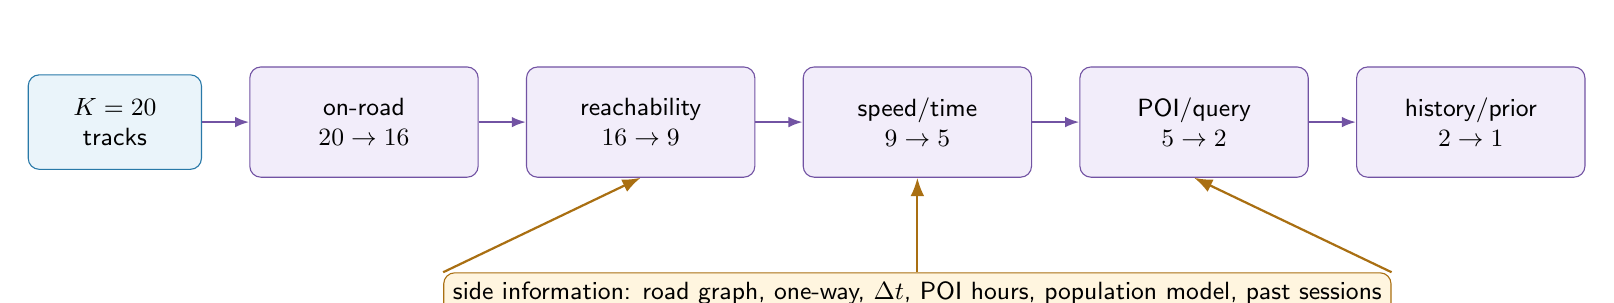
\begin{tikzpicture}[
  font=\small\sffamily,
  stage/.style={draw=purple,fill=lightpurple,rounded corners,minimum width=29mm,minimum height=14mm,align=center},
  n/.style={draw=blue,fill=lightblue,rounded corners,minimum width=22mm,minimum height=12mm,align=center},
  arr/.style={-{Latex[length=1.8mm]},thick,draw=purple}
]
\node[n] (k) {$K=20$\\tracks};
\node[stage,right=6mm of k] (road) {on-road\\$20\to16$};
\node[stage,right=6mm of road] (reach) {reachability\\$16\to9$};
\node[stage,right=6mm of reach] (time) {speed/time\\$9\to5$};
\node[stage,right=6mm of time] (poi) {POI/query\\$5\to2$};
\node[stage,right=6mm of poi] (hist) {history/prior\\$2\to1$};
\draw[arr] (k)--(road); \draw[arr] (road)--(reach); \draw[arr] (reach)--(time);
\draw[arr] (time)--(poi); \draw[arr] (poi)--(hist);
\node[draw=amber,fill=lightamber,rounded corners,align=center,below=12mm of time] (side)
  {side information: road graph, one-way, $\Delta t$, POI hours, population model, past sessions};
\draw[-{Latex},thick,amber] (side.north)--(time.south);
\draw[-{Latex},thick,amber] (side.north west)--(reach.south);
\draw[-{Latex},thick,amber] (side.north east)--(poi.south);
\end{tikzpicture}}
\caption{Ví dụ attack funnel: 20 output không có nghĩa là 20 giả thuyết còn sống sau ngữ cảnh. Các con số chỉ minh họa, không phải kết quả thực nghiệm.}
\label{fig:attack-funnel}
\end{figure}

\subsection{Các nguồn ngữ cảnh chính}

\begin{description}
  \item[Bản đồ và map matching] Loại điểm ngoài đường, đường cấm hoặc đoạn không
  liên thông với lịch sử gần nhất.
  \item[Không gian--thời gian] Dùng giới hạn tốc độ, thời gian di chuyển, hướng và
  xác suất transition để nối các frame.
  \item[POI và semantics] Giờ mở cửa, loại POI, thói quen theo thời điểm và query
  content giúp xếp hạng điểm dừng.
  \item[Population prior] Mô hình OD, mật độ, tuyến phổ biến và traffic làm một số
  candidate có prior lớn hơn.
  \item[Lịch sử cá nhân] Home/work, trajectory cũ, device fingerprint và pattern
  phiên giúp link batch với người dùng.
\end{description}

Survey Chow--Mokbel đã dự báo rõ rủi ro semantic/background information đối với
personalized LBS: khi biết sở thích và lịch sinh hoạt, đối thủ có thể suy ra điểm
thật trong một vùng cloak với độ chắc chắn cao hơn \cite{chow2011trajectory}. Đây
là cầu nối trực tiếp từ nền tảng Mokbel đến threat model context-aware hiện tại.

\section{Task của attacker phụ thuộc output contract}

\begin{table}[htbp]
\centering
\small
\caption{Không dùng metric membership cho một output không chứa truth.}
\label{tab:contract-task-metric}
\begin{tabularx}{\textwidth}{P{3.0cm}P{4.2cm}Y}
\toprule
\textbf{Output contract} & \textbf{Attacker task đúng} & \textbf{Metric phù hợp}\\
\midrule
Truth $+$ dummies & Chọn/xếp hạng member thật & Top-1 accuracy, rank/MRR, posterior của truth, survival rate\\
Một output thay thế & Tái dựng $x_t$ hoặc $T$ & Expected inference error, success trong bán kính $r$, attack DTW\\
Dummy-only tracks & Tái dựng/link secret từ toàn batch & EIE, reconstruction success, advantage trên prior, identity/route leakage\\
Cloaked region & Xác định người/điểm trong vùng & Effective anonymity, posterior entropy, query-linking success\\
\bottomrule
\end{tabularx}
\end{table}

Trong real-in-set, rank của truth có nghĩa vì truth là một phần tử quan sát. Trong
dummy-only, hỏi ``truth đứng thứ mấy trong batch?'' là sai kiểu dữ liệu; cần một
reconstructor tạo $\hat{x}_t$ hoặc $\hat{T}$ từ batch rồi so với secret chỉ ở evaluator.

\section{Bốn nhóm metric cần báo cáo cùng nhau}

\subsection{Privacy dưới attacker cụ thể}

\begin{itemize}
  \item \textbf{Top-1/Top-$r$ success:} attacker chọn đúng member hoặc tái dựng trong ngưỡng.
  \item \textbf{Expected Inference Error (EIE):}
  $\mathbb{E}[d(X,\hat X(O,C_A))]$; lớn hơn thường tốt cho privacy.
  \item \textbf{Posterior entropy:} $H(X\mid O,C_A)=-\sum_xp(x)\log p(x)$; phải dùng
  posterior của attacker, không phải entropy hình học của output.
  \item \textbf{Attacker advantage:} chênh lệch so với attacker chỉ có prior; tránh
  tuyên bố thành công khi defense không tốt hơn baseline ngây thơ.
\end{itemize}

\subsection{Plausibility/survival}

Tỷ lệ on-road, transition hợp lệ, tốc độ hợp lệ, semantic likelihood và số giả
thuyết sống sau mỗi stage cho biết \emph{vì sao} attacker thành công. Đây là
diagnostic metric, không thay cho outcome privacy.

\subsection{Utility của ứng dụng}

Với query POI, có thể đo top-$k$ POI overlap/recall, thứ hạng POI thật, khoảng cách
đến POI được trả, route/travel-time error và task success. Metric phải bắt chước
dịch vụ thực tế. Khoảng cách perturbation đơn thuần không biết người dùng còn tìm
được đúng bệnh viện/cửa hàng hay không.

\subsection{Overhead}

Số request, byte upload/download, server queries, latency, CPU, memory và energy.
Real-in-set với $K$ candidates thường nhân khối lượng query; Casper tăng candidate
answer; dummy-only cần chỉ rõ cách client lấy được dịch vụ hữu ích từ batch.

\begin{figure}[htbp]
\centering
\begin{tikzpicture}[font=\small\sffamily]
\coordinate (A) at (0,0); \coordinate (B) at (7,0); \coordinate (C) at (3.5,5.5);
\draw[navy,very thick] (A)--(B)--(C)--cycle;
\fill[lightpurple] (A) circle (9mm); \node[purple,font=\bfseries,align=center] at (A) {Privacy\\attacker};
\fill[lightgreen] (B) circle (9mm); \node[green,font=\bfseries,align=center] at (B) {Utility\\task};
\fill[lightamber] (C) circle (9mm); \node[amber,font=\bfseries,align=center] at (C) {Overhead\\system};
\node[navy,align=center] at (3.5,2.0) {Một kết quả đầy đủ\\phải báo cáo cả ba};
\end{tikzpicture}
\caption{Privacy--utility--overhead là ba trục, không phải một số duy nhất để tối ưu.}
\label{fig:metric-triangle}
\end{figure}

\begin{warningbox}
``Entropy cao'', ``DD lớn'', ``đủ $K$ track'' hoặc ``tất cả điểm nằm trên đường''
chỉ là tín hiệu trung gian. Không metric nào trong số đó tự chứng minh attacker
không tái dựng được truth hoặc người dùng vẫn nhận đúng dịch vụ.
\end{warningbox}

\begin{exercisebox}
Một defense tăng EIE từ 300 m lên 900 m nhưng POI recall@5 giảm từ 0.92 xuống
0.18 và request bytes tăng 10 lần. Hãy viết một kết luận trung lập. Có thể gọi đây
là ``tốt hơn'' nếu chưa định nghĩa utility/overhead budget không?
\end{exercisebox}

% ============================================================================
\chapter{Geo-Indistinguishability: bảo đảm xác suất khác với ẩn trong nhóm}

\section{Trực giác likelihood ratio theo khoảng cách}

Geo-Indistinguishability (Geo-I) áp dụng ý tưởng differential privacy cho vị trí
metric \cite{andres2013geo}. Với kernel $K$ và mọi tập đầu ra đo được $Z$:
\[
K(x)(Z)\le e^{\varepsilon d(x,x')}K(x')(Z).
\]
Hai vị trí thật $x,x'$ càng gần nhau thì phân phối output phải càng khó phân biệt.
$\varepsilon$ nhỏ làm ràng buộc chặt hơn; nhưng output thường xa truth hơn và utility
giảm. Ý nghĩa phải đi cùng đơn vị: nếu $d$ tính bằng kilomet thì $\varepsilon$ có
đơn vị km$^{-1}$.

\begin{figure}[htbp]
\centering
\begin{tikzpicture}[font=\small\sffamily,x=1cm,y=1cm]
  \fill[lightblue,opacity=.85] (3,2.6) circle (2.25);
  \fill[lightpurple,opacity=.65] (6,2.6) circle (2.25);
  \fill[blue] (3,2.6) circle (3pt); \node[blue,below] at (3,2.4) {$x$};
  \fill[purple] (6,2.6) circle (3pt); \node[purple,below] at (6,2.4) {$x'$};
  \draw[<->,thick,graytext] (3,2.6)-- node[above] {$d(x,x')$} (6,2.6);
  \node[blue,align=center] at (1.1,5.2) {phân phối\\output từ $x$};
  \node[purple,align=center] at (7.9,5.2) {phân phối\\output từ $x'$};
  \node[navy,align=center] at (4.5,.1) {vùng chồng lấp lớn $\Rightarrow$\\khó biết secret nào sinh output};
\end{tikzpicture}
\caption{Trực giác Geo-I: đây là quan hệ giữa hai phân phối đầu ra, không phải số lượng candidate trong một lần chạy.}
\label{fig:geo-i-overlap}
\end{figure}

\section{Planar Laplace: bán kính không phải Exponential}

Trong mặt phẳng Euclid, cơ chế planar Laplace có mật độ theo diện tích
\[
f(z\mid x)=\frac{\varepsilon^2}{2\pi}
\exp\bigl(-\varepsilon\lVert z-x\rVert_2\bigr).
\]
Khi đổi sang tọa độ cực, phần tử diện tích thêm hệ số $r$, nên bán kính có mật độ
\[
f_R(r)=\varepsilon^2 r e^{-\varepsilon r},\qquad r\ge0,
\]
tức $R\sim\operatorname{Gamma}(\text{shape}=2,\text{scale}=1/\varepsilon)$ và
$\mathbb{E}[R]=2/\varepsilon$. Góc $\Theta$ uniform trên $[0,2\pi)$.

\begin{warningbox}[Lỗi quan trọng trong Internship 2 cũ]
Lấy $R\sim\operatorname{Exponential}(\varepsilon)$ rồi chọn góc đều \textbf{không}
tạo planar Laplace theo công thức trên: nó thiếu hệ số Jacobian $r$. Bản luận văn
hiện tại cần nói rõ kernel nào được dùng và proof thuộc kernel lý tưởng hay sampler
số thực cụ thể.
\end{warningbox}

\section{Geo-I không phải \texorpdfstring{$k$}{k}-anonymity}

\begin{table}[htbp]
\centering
\small
\caption{So sánh hai kiểu bảo đảm.}
\label{tab:k-vs-geoi}
\begin{tabularx}{\textwidth}{P{3.2cm}Y Y}
\toprule
 & \textbf{$k$-anonymity/spatial cloaking} & \textbf{Geo-I}\\
\midrule
Đối tượng & Nhóm/lớp tương đương hoặc vùng chứa người & Phân phối randomized output\\
Tham số & $k$, $A_{\min}$ (và constraint utility) & $\varepsilon$ cùng metric $d$\\
Phụ thuộc population & Thường có & Không cần người khác đang ở gần để định nghĩa\\
Claim & Ít nhất $k$ đối tượng giống nhau theo representation & Likelihood ratio bị chặn theo khoảng cách\\
Yếu điểm & Prior/semantic, homogeneity, tracking & Composition, correlation, model mismatch, utility\\
Không nói gì về & Mọi posterior tùy ý & Realism, on-roadness, query-content/identity tự động\\
\bottomrule
\end{tabularx}
\end{table}

Không tồn tại phép đổi chung ``$k=10$ tương đương $\varepsilon=0.2$''. Hai tham số
đo hai đối tượng toán học khác nhau. Cũng không thể chứng minh Geo-I bằng cách
chỉ quan sát rằng một batch có nhiều dummy.

\section{Post-processing và điểm dễ gãy}

Nếu $A=M(X)$ đã thỏa Geo-I và tầng sau tạo $O=G(A,C_{pub};R_G)$ mà không truy cập
lại $X$, thì $O$ thừa hưởng bảo đảm qua post-processing. Sơ đồ cần kiểm tra là
\[
X\xrightarrow{\;M_{\varepsilon}\;}A
\xrightarrow{\;G(\cdot,C_{pub})\;}O.
\]

\begin{figure}[htbp]
\centering
\resizebox{.96\textwidth}{!}{%
\begin{tikzpicture}[
 font=\small\sffamily,node distance=9mm,
 s/.style={draw=red,fill=lightred,rounded corners,minimum width=34mm,minimum height=13mm,align=center},
 m/.style={draw=green,fill=lightgreen,rounded corners,minimum width=34mm,minimum height=13mm,align=center},
 o/.style={draw=blue,fill=lightblue,rounded corners,minimum width=40mm,minimum height=13mm,align=center},
 bad/.style={draw=red,dashed,-{Latex[length=2mm]},thick},
 arr/.style={-{Latex[length=2mm]},thick,draw=graytext}
]
\node[s] (x) {secret\\$x_t$};
\node[m,right=of x] (rem) {kernel riêng tư\\anchor $a_t$};
\node[m,right=of rem] (g) {generator\\public context};
\node[o,right=of g] (out) {$K$ stable\\dummy tracks};
\draw[arr] (x)--(rem); \draw[arr] (rem)--(g); \draw[arr] (g)--(out);
\draw[bad,bend right=38] (x.south) to node[below,font=\scriptsize,align=center]{đọc lại truth\\$\Rightarrow$ proof gãy} (g.south);
\end{tikzpicture}}
\caption{Post-processing chỉ hợp lệ khi generator thật sự chỉ phụ thuộc anchor, dữ liệu công khai và randomness thích hợp.}
\label{fig:post-processing}
\end{figure}

Các điểm cần audit trong code/proof:

\begin{itemize}
  \item generator có đọc truth, distance-to-truth hoặc nhãn truth để reject candidate không;
  \item randomness tầng sau có độc lập theo điều kiện cần thiết hay bị dùng chung state
  khiến distribution phụ thuộc số vòng rút secret-dependent;
  \item map matching/projection là deterministic post-processing của output hay quay
  lại chọn theo exact location;
  \item implementation float64/discrete sampler có đúng kernel được chứng minh không.
\end{itemize}

\section{Một event khác cả trajectory}

Paper Geo-I gốc có thảo luận tuple/set; riêng planar mechanism cơ sở vẫn bảo vệ một
điểm. Với $n$ điểm lấy mẫu độc lập, bound nêu trong nguồn tăng thành $n\varepsilon$
dưới metric tuple thích hợp. Nói tổng quát, nếu mỗi lần phát hành thỏa
$\varepsilon_t$-Geo-I, một bound composition cơ bản cho toàn transcript cộng dồn
thành $\sum_t\varepsilon_t$. Temporal correlation còn có thể giúp attacker hơn nữa
nếu threat model không nằm trọn trong guarantee. Vì vậy:

\begin{itemize}
  \item \textbf{per-event Geo-I} không được gọi thành trajectory-level privacy;
  \item cần privacy budget/schedule và định nghĩa adjacency cho trajectory;
  \item cần attacker evaluation trên toàn sequence, không chỉ histogram của một step.
\end{itemize}

\begin{exercisebox}
Một ứng dụng phát hành 60 lần, mỗi lần dùng $\varepsilon=0.1$ km$^{-1}$. Bound cộng
đơn giản là bao nhiêu? Tại sao việc từng output ``trông nhiễu'' không đủ để nói cả
phiên có cùng mức 0.1? Nếu generator đọc lại truth để giữ dummy cách truth 500 m,
ta còn viện dẫn post-processing được không?
\end{exercisebox}


% ============================================================================
\chapter{Đặt các lớp giải pháp cạnh nhau}

\section{Một bảng so sánh theo đúng sáu câu hỏi}

\begin{table}[htbp]
\centering
\scriptsize
\caption{So sánh các họ cơ chế; dấu ``---'' nghĩa là không có bảo đảm mặc định, không phải cơ chế vô dụng.}
\label{tab:family-comparison}
\begin{tabularx}{\textwidth}{P{2.25cm}P{2.2cm}P{2.3cm}P{2.45cm}Y}
\toprule
\textbf{Họ} & \textbf{LSP thấy} & \textbf{Tin cậy} & \textbf{Claim điển hình} & \textbf{Giới hạn nổi bật}\\
\midrule
Spatial cloaking/Casper & vùng + query & anonymizer & $k$ người thật, $A_{\min}$ & prior, tracking, vùng lớn, bên trung gian\\
P2P cloaking & vùng + query & các peer phối hợp & $k$ người thật trong vùng; chống center estimator cụ thể & peer leakage, partition, snapshot\\
Mix-zone & pseudonym trước/sau vùng trộn & mix-zone/điều kiện traffic & unlinkability cục bộ & timing/road constraints; đổi ID có thể phá service\\
Path confusion & một số location samples & cơ chế phát hành & tracking uncertainty/ngưỡng confusion & phụ thuộc tracker model, bỏ mẫu ảnh hưởng utility\\
Real-in-set dummy & truth $+$ dummy & client & ambiguity theo set/metric & filterability, overhead, truth là member\\
Replacement/noise & một output đã nhiễu & client & có thể là Geo-I & giảm query utility, composition\\
Dummy-only thesis & $K$ fake tracks & client & post-processing có điều kiện từ anchor & không phải $k$-anon; utility/reconstruction chưa tự có\\
\bottomrule
\end{tabularx}
\end{table}

\section{Ba kiến trúc cần phân biệt bằng một cái nhìn}

\begin{figure}[htbp]
\centering
\resizebox{\textwidth}{!}{%
\begin{tikzpicture}[
 font=\scriptsize\sffamily,
 device/.style={draw=green,fill=lightgreen,rounded corners,minimum width=28mm,minimum height=12mm,align=center},
 process/.style={draw=navy,fill=lightblue,rounded corners,minimum width=31mm,minimum height=12mm,align=center},
 server/.style={draw=red,fill=lightred,rounded corners,minimum width=28mm,minimum height=12mm,align=center},
 arr/.style={-{Latex[length=1.8mm]},thick,draw=graytext}
]
\node[font=\small\bfseries] at (3.0,5.0) {A. LBS trực tiếp};
\node[device] (a1) at (1.2,3.8) {client\\$x,q$};
\node[server] (a2) at (4.8,3.8) {LSP\\thấy truth};
\draw[arr,red] (a1)-- node[above]{exact request} (a2);

\node[font=\small\bfseries] at (9.3,5.0) {B. Casper};
\node[device] (b1) at (6.8,3.8) {client\\truth};
\node[process] (b2) at (9.3,3.8) {trusted\\anonymizer};
\node[server] (b3) at (12.0,3.8) {LSP\\region};
\draw[arr] (b1)--(b2); \draw[arr] (b2)--(b3);
\node[process] (b4) at (9.3,2.1) {candidate\\refinement};
\draw[arr] (b3.south) |- (b4.east); \draw[arr] (b4.west) -| (b1.south);

\node[font=\small\bfseries] at (16.1,5.0) {C. Dummy-only thesis};
\node[device] (c1) at (14.0,3.8) {client\\truth};
\node[process] (c2) at (16.6,3.8) {anchor $+$\\generator};
\node[server] (c3) at (19.2,3.8) {LSP\\fake batch};
\draw[arr] (c1)--(c2); \draw[arr] (c2)--(c3);
\node[draw=purple,fill=lightpurple,rounded corners,align=center] at (16.6,2.0)
  {cần định nghĩa riêng\\cách giữ utility};
\end{tikzpicture}}
\caption{Khác biệt cốt lõi nằm ở trust boundary, output contract và cách lấy đáp án hữu ích; không chỉ ở hình dạng noise.}
\label{fig:three-architectures}
\end{figure}

\section{Những điều các nguồn Mokbel không chứng minh}

Các công trình Mokbel/Chow là nền tảng quan trọng về kiến trúc, query processing,
continuous attacks và taxonomy. Tuy nhiên, chúng \textbf{không} tự cung cấp bằng
chứng cho các claim sau:

\begin{itemize}
  \item một cơ chế năm 2026 là SOTA;
  \item dummy-only đạt spatial $k$-anonymity hay membership success $1/K$;
  \item Geo-I, differential privacy hoặc composition cho quỹ đạo;
  \item chống mọi Bayesian attacker có map/time/POI/population prior;
  \item POI top-$k$ utility là ``industry standard'' phổ quát;
  \item query-coordinate privacy tự động bảo vệ semantic query content;
  \item một commercial deployment thực tế của Casper.
\end{itemize}

\begin{sourcebox}
Chow--Mokbel 2011 là survey hệ thống hóa lĩnh vực. Nguồn gốc $k$-anonymity thuộc
Samarati/Sweeney; SD--TD--DD thuộc You--Peng--Lee; Geo-I thuộc Andrés và cộng sự.
The New Casper/Casper* là đóng góp kiến trúc và query processing của
Mokbel--Chow--Aref. Gán đúng công lao cũng giúp ta gán đúng phạm vi của claim.
\end{sourcebox}

% ============================================================================
\chapter{Nối kiến thức nền với luận văn hiện tại}

\section{Luận văn đang đứng ở đâu trong bản đồ?}

Kiến trúc hiện tại có thể cô đọng như sau:
\[
x_t
\xrightarrow{\text{REM lý tưởng, }\varepsilon_t}
a_t
\xrightarrow{G_K(a_{1:t},C_{pub})}
\mathcal D_t=\{D_{1,1:t},\ldots,D_{K,1:t}\}.
\]
Thiết bị giữ $x_t$; một kernel lấy anchor $a_t$; generator dùng anchor, mạng đường,
public context và randomness để tạo $K$ stable dummy tracks; LSP quan sát batch giả.

\begin{thesisbox}
Luận văn thuộc lớp \textbf{on-device, dummy-only trajectory protection có một
privacy anchor}, không phải Casper, không phải classical truth-in-set dummy và
không phải trajectory data publication. Mokbel cung cấp nền tảng để hiểu kiến trúc,
tracking attack và semantic side information; claim cuối phải được chứng minh riêng
cho output contract này.
\end{thesisbox}

\section{Bốn mức độ claim phải giữ tách biệt}

\begin{table}[htbp]
\centering
\small
\caption{Thang bằng chứng cho luận văn hiện tại.}
\label{tab:claim-ladder}
\begin{tabularx}{\textwidth}{P{3.3cm}Y Y}
\toprule
\textbf{Mức} & \textbf{Có thể nói gì?} & \textbf{Cần tránh nói quá}\\
\midrule
Đã hiện thực & Output dummy-only, stable track IDs, map-aware generation, ranh giới secret/evaluator & Không biến integration demo thành privacy result\\
Lập luận có điều kiện & Post-processing của ideal REM nếu generator không đọc lại secret & Không suy ra cho float64 sampler/toàn trajectory nếu chưa proof\\
Đang cần chứng minh & Chống context-aware reconstruction, POI utility, population prior, repeated trials & Không gọi ``privacy-preserving'' như kết luận đã đóng\\
Ngoài claim hiện tại & Semantic query-content privacy, identity unlinkability, active LSP protocol & Không gom vào một từ ``trajectory privacy'' chung chung\\
\bottomrule
\end{tabularx}
\end{table}

\section{``Group of users'' trong Mokbel khác gì hướng thesis?}

Trong paper continuous queries, dynamic group là \textbf{những người thật đang tồn
tại đồng thời} và cùng chia sẻ cloaked region; memorization giữ nhóm ban đầu trong
những snapshot sau \cite{chow2007continuous}. Nó không đồng nghĩa với:

\begin{itemize}
  \item population prior học từ nhiều trajectory lịch sử;
  \item group differential privacy;
  \item pooling dữ liệu nhiều người để train generator;
  \item tạo $K$ dummy từ một client.
\end{itemize}

Nếu thesis ``kết hợp group of users'', phải chọn một nghĩa và vẽ data flow/trust
boundary lại. Dùng population statistics công khai để làm dummy plausible là một
hướng khác với buộc nhiều người thật cùng phát hành một vùng.

\section{Ma trận câu hỏi để review từng phần luận văn}

\begin{longtable}{P{1.2cm}P{4.2cm}P{5.0cm}P{3.7cm}}
\caption{Checklist review khoa học, dùng trực tiếp khi đọc bản graduation thesis.}
\label{tab:review-checklist}\\
\toprule
\textbf{ID} & \textbf{Câu hỏi} & \textbf{Bằng chứng phải thấy} & \textbf{Dấu hiệu lỗi}\\
\midrule
\endfirsthead
\toprule
\textbf{ID} & \textbf{Câu hỏi} & \textbf{Bằng chứng phải thấy} & \textbf{Dấu hiệu lỗi}\\
\midrule
\endhead
R1 & Secret, output và trusted components đã rõ chưa? & Sơ đồ system model + data contract & Dùng ``location data'' chung chung\\
R2 & Snapshot hay continuous? & Transcript $O_{1:T}$, state, stable identity & Chỉ đánh giá từng điểm độc lập\\
R3 & Online LBS hay offline publication? & Query protocol/latency hoặc release model & Trộn synthetic dataset với online request\\
R4 & $k/K$ đếm cái gì? & Real users, candidates hay tracks được nói rõ & Gọi mọi tập $K$ là $k$-anonymous\\
R5 & Attacker biết gì? & Map, time, POI, algorithm, prior, history & Attacker chỉ ``nhìn bằng mắt''\\
R6 & Attack task khớp output chưa? & Membership hoặc reconstruction được định nghĩa & Rank truth khi truth không trong batch\\
R7 & Geo-I claim ở mức nào? & Kernel, metric, units, adjacency, composition & Từ per-event suy ra cả trajectory\\
R8 & Post-processing có thật không? & Code/dataflow không đọc lại truth & Reject/score candidate bằng truth\\
R9 & Utility là task thực tế nào? & POI/routing task + ground-truth query & Chỉ dùng Euclidean displacement\\
R10 & Kết quả có uncertainty? & Nhiều seeds/users/scenarios + CI & Một xe, một seed, một demo\\
R11 & Comparator có cùng contract? & Adapter và limitation table & So số trực tiếp giữa truth-in-set và dummy-only\\
R12 & Claim có đúng nguồn? & Primary citation + phạm vi paper & Survey bị biến thành proof/SOTA\\
\bottomrule
\end{longtable}

\section{Ba câu trình bày ngắn cho buổi gặp thầy}

\begin{takeaway}[30 giây: nền tảng]
$k$-anonymity là tiêu chí ẩn danh trong một nhóm; spatial cloaking tạo vùng chứa
người thật; Casper ghép anonymizer với query processor để vẫn trả đáp án đúng.
Dummy generation là một họ khác: client tạo các khả năng giả, và privacy chỉ tồn
tại nếu attacker dùng map, time, POI và history vẫn không lọc được chúng.
\end{takeaway}

\begin{takeaway}[30 giây: khoảng trống mà thesis nhắm tới]
Các dummy cổ điển thường được đánh giá bằng set size, khoảng cách hoặc mô hình
attacker đơn giản. Thesis tập trung vào việc dummy bị lọc xuyên thời gian bởi tính
khả đạt và ngữ cảnh, rồi đo privacy bằng reconstruction attack cùng utility của
truy vấn POI thay vì chỉ một QoS tự định nghĩa.
\end{takeaway}

\begin{takeaway}[30 giây: claim trung thực hiện tại]
Hệ thống hiện tạo được $K$ stable dummy-only tracks từ một anchor riêng tư trên
mạng đường. Bảo đảm Geo-I mới là lập luận có điều kiện cho kernel REM lý tưởng theo
từng event; chống attacker ngữ cảnh, utility POI và trajectory-level composition là
những phần phải thực nghiệm và chứng minh tiếp.
\end{takeaway}

\begin{exercisebox}
Tự thu âm ba đoạn trên. Nếu một đoạn dài quá 40 giây, bỏ chi tiết implementation;
nhưng không bỏ output contract, attacker hoặc giới hạn claim. Đó là ba điểm giúp
giáo viên phân biệt thesis với Casper và dummy cổ điển.
\end{exercisebox}


% ============================================================================
\appendix
\chapter{Lộ trình đọc paper và materials}

\section{Đọc theo câu hỏi, không đọc theo năm}

\begin{longtable}{P{3.3cm}P{3.0cm}P{5.0cm}P{3.0cm}}
\caption{Lộ trình đọc ưu tiên; mọi đường dẫn là bản chính thức hoặc author-hosted.}
\label{tab:reading-route}\\
\toprule
\textbf{Nguồn} & \textbf{Đọc phần nào trước} & \textbf{Câu hỏi cần trả lời} & \textbf{Đừng gán nhầm}\\
\midrule
\endfirsthead
\toprule
\textbf{Nguồn} & \textbf{Đọc phần nào trước} & \textbf{Câu hỏi cần trả lời} & \textbf{Đừng gán nhầm}\\
\midrule
\endhead
\href{https://www.kdd.org/exploration_files/v13-01-5-mokbel.pdf}{Chow--Mokbel 2011} & Sec. 1--3.5, 5 & Snapshot/continuous; taxonomy; SD--TD--DD; semantic risk & Survey không phát minh mọi kỹ thuật\\
\href{https://www.vldb.org/conf/2006/p763-mokbel.pdf}{The New Casper 2006} & Sec. 1, 3--5 & Anonymizer và query processor phối hợp ra sao? & Casper không phải dummy\\
\href{https://dmlab.cs.umn.edu/new/papers/tods09.pdf}{Casper* 2009} & Sec. 3--5 & Ba query classes; candidate answers; continuous/shared execution & Query correctness không phải Geo-I\\
\href{https://dmlab.cs.umn.edu/new/papers/SSTD07.pdf}{Chow--Mokbel 2007} & Sec. 3--6 & $k_l/k_q$; sampling/tracking; sharing/memorization & Query privacy ở đây là issuer unlinkability\\
\href{https://dmlab.cs.umn.edu/new/papers/geoinformatica10.pdf}{P2P cloaking 2011} & Sec. 3--5 & Không có anonymizer thì peer phối hợp thế nào? & Center attack defense là attack-specific\\
\href{https://dmlab.cs.umn.edu/new/papers/geoinformatica10b.pdf}{Road-network cloaking 2011} & Sec. 3--5 & Vì sao rectangle Euclid không đủ trên mạng đường? & Road cloak không phải dummy/Geo-I\\
\href{https://www.cse.psu.edu/~wul2/Publications/wlee%20palms2007.pdf}{You--Peng--Lee 2007} & Toàn bài (5 trang) & Dummy track dài hạn và SD--TD--DD được định nghĩa thế nào? & Truth nằm trong tập; metric dùng model cũ\\
\href{https://doi.org/10.1145/2508859.2516735}{Andrés et al. 2013} & Sec. 2--4 & Metric privacy, planar Laplace, utility trade-off & Per-event không phải trajectory guarantee\\
\bottomrule
\end{longtable}

\section{Liên hệ đúng với Internship 2}

Trong \code{archive/internship\_2/report.pdf}, phần liên quan Chow--Mokbel nằm ở physical
pages 15--17 (printed pages 10--12); bibliography nằm ở physical page 42. Phần đó
hỗ trợ snapshot/continuous, taxonomy cloaking--mix-zone--path-confusion--dummy và
online/publication. Nó \textbf{không} trình bày đầy đủ pipeline Casper, nên tài liệu
này bổ sung từ các paper gốc thay vì coi kiến thức đó đã có trong Internship 2.

\begin{warningbox}[Lưu ý khi đọc source Internship 2 đã lưu trữ]
Entry cũ \code{chow2011trajectory} trong
\code{archive/internship\_2/thesis/refs.bib} ghi
\code{@inproceedings}, venue SPRINGL và trang 13--20. Hãy đổi sang journal
\emph{ACM SIGKDD Explorations Newsletter}, 13(1), 19--29, 2011, DOI
\href{https://doi.org/10.1145/2031331.2031335}{10.1145/2031331.2031335}.
Bibliography tự chứa của \code{thesis/main.tex} đã dùng metadata đúng.
\end{warningbox}

\chapter{Đáp án ngắn cho phần tự kiểm tra}

\begin{enumerate}
  \item \textbf{Khung sáu biến.} Secret có thể là $x_{1:T}$, identity và $q_{1:T}$;
  LSP thấy five-point batch, pseudonym và timing; side information gồm map, speed,
  POI, history và population prior. Câu $1/5$ đã bỏ qua likelihood và prior trong Bayes.

  \item \textbf{$k$ và $A_{\min}$.} $k=10$ chỉ nói số người, không ngăn vùng rất
  nhỏ. $A_{\min}$ buộc vùng vượt khỏi cửa hàng. Vùng lớn làm nhiều bệnh viện có
  thể là nearest cho một điểm nào đó, nên candidate list/bandwidth/refinement tăng.

  \item \textbf{Casper 30 giây.} Client gửi truth cho trusted anonymizer; anonymizer
  tạo cloaked region; LSP trả candidate list cho toàn vùng; phía tin cậy refinement
  bằng truth. Thiếu một mắt xích thì hoặc lộ vị trí, hoặc không có cách bảo toàn đáp án.

  \item \textbf{Continuous intersection.} Giao ba tập là $\{A,C\}$, còn hai người.
  Nếu chỉ đường của $A$ khả thi thì anonymity hiệu dụng còn một. Memorization giữ
  thành viên trong vùng nhưng không tự làm mọi path động học đều hợp lý.

  \item \textbf{Dummy filtering.} Sau filter chỉ một track sống, nên effective
  ambiguity gần 1 dù $K=5$. DD vẫn có thể rất cao vì bốn track vô lý nằm xa truth;
  điều đó minh họa DD không phải privacy outcome.

  \item \textbf{Trade-off metric.} Có thể nói defense tăng sai số của attacker nhưng
  gây suy giảm utility và overhead lớn. Chưa có budget/weight hay Pareto criterion
  thì không đủ cơ sở gọi tổng thể ``tốt hơn''.

  \item \textbf{Geo-I composition.} Bound cộng cơ bản là $60\times0.1=6$
  km$^{-1}$. Nhiều lần quan sát tạo transcript khác một event. Generator đọc lại
  truth để enforce 500 m không còn là post-processing chỉ của private anchor.

  \item \textbf{Ba đoạn trình bày.} Một câu trả lời đạt yêu cầu nếu gọi đúng output
  contract, attacker task, phạm vi proof và phần empirical evidence còn thiếu; không
  cần kể chi tiết từng class/code file.
\end{enumerate}

\chapter{Bảng thuật ngữ nhanh}

\begin{longtable}{P{3.5cm}P{10.7cm}}
\caption{Thuật ngữ dùng nhất quán trong tài liệu.}\label{tab:glossary}\\
\toprule
\textbf{Thuật ngữ} & \textbf{Nghĩa sử dụng}\\
\midrule
\endfirsthead
\toprule
\textbf{Thuật ngữ} & \textbf{Nghĩa sử dụng}\\
\midrule
\endhead
LBS & Dịch vụ dựa trên vị trí.\\
LSP & Nhà cung cấp/dịch vụ xử lý request vị trí; thường nằm ngoài trust boundary.\\
LPPM & Cơ chế bảo vệ riêng tư vị trí trước hoặc trong quá trình dùng dịch vụ.\\
Quasi-identifier & Thuộc tính không phải tên trực tiếp nhưng có thể link với nguồn phụ để nhận diện.\\
Anonymity set & Tập các đối tượng/giả thuyết mà attacker còn coi là có thể.\\
Spatial cloaking & Thay exact point bằng một spatial region.\\
Casper & Framework có location anonymizer và privacy-aware query processor.\\
Dummy & Vị trí/quỹ đạo giả; phải chỉ rõ replacement, real-in-set hay dummy-only.\\
Stable track & Chuỗi dummy giữ ID và chuyển động nhất quán qua thời gian.\\
Prior & Phân phối niềm tin của attacker trước khi xem output mới.\\
Posterior & Phân phối sau khi kết hợp output với prior/side information.\\
Geo-I & Bảo đảm likelihood-ratio theo metric distance giữa hai secret locations.\\
REM & Exponential mechanism rời rạc; trong thesis dùng để tạo private anchor trên support.\\
EIE & Expected inference error của attacker.\\
POI utility & Chất lượng task POI, ví dụ overlap/recall/rank của kết quả cần thiết.\\
Output contract & Cấu trúc chính xác mà LSP quan sát; quyết định attacker task và metric.\\
\bottomrule
\end{longtable}

\chapter*{Kết luận học tập}
\addcontentsline{toc}{chapter}{Kết luận học tập}

Nếu chỉ giữ lại năm ý, hãy giữ các ý sau:

\begin{enumerate}
  \item $k$-anonymity là một \textbf{tiêu chí}, spatial cloaking là một
  \textbf{cơ chế}, Casper là một \textbf{kiến trúc}.
  \item Spatial $k$-anonymity dựa vào \textbf{người thật}; $K$ dummy là candidate
  do một client sinh. Cùng ký tự nhưng không cùng bảo đảm.
  \item Privacy snapshot không tự kéo dài sang trajectory: intersection, reachability,
  semantic và history làm anonymity set co lại.
  \item Dummy tốt là dummy sống sót trước attacker có ngữ cảnh; SD, TD và DD là
  nền tảng lịch sử nhưng không thay calibrated attack evaluation.
  \item Geo-I giới hạn quan hệ giữa \textbf{phân phối output}; nó không tự bảo đảm
  realism, utility, identity/query-content privacy hay cả trajectory qua nhiều release.
\end{enumerate}

Từ nền tảng này, việc review graduation thesis nên bắt đầu bằng data contract và
threat model, sau đó mới kiểm tra proof, attacker, utility và kết quả. Nếu năm lớp
đó ăn khớp, implementation mới có ý nghĩa khoa học rõ ràng.

\clearpage
\begin{thebibliography}{99}
\small

\bibitem{chow2011trajectory}
Chi-Yin Chow and Mohamed F. Mokbel.
\newblock Trajectory privacy in location-based services and data publication.
\newblock \emph{ACM SIGKDD Explorations Newsletter}, 13(1):19--29, 2011.
\newblock DOI: \href{https://doi.org/10.1145/2031331.2031335}{10.1145/2031331.2031335}.

\bibitem{mokbel2006casper}
Mohamed F. Mokbel, Chi-Yin Chow, and Walid G. Aref.
\newblock The New Casper: Query processing for location services without compromising privacy.
\newblock In \emph{Proceedings of the 32nd International Conference on Very Large Data Bases (VLDB)}, pages 763--774, 2006.
\newblock DOI: \href{https://doi.org/10.5555/1182635.1164193}{10.5555/1182635.1164193};
official paper: \href{https://www.vldb.org/conf/2006/p763-mokbel.pdf}{VLDB Endowment PDF}.

\bibitem{chow2009casper}
Chi-Yin Chow, Mohamed F. Mokbel, and Walid G. Aref.
\newblock Casper*: Query processing for location services without compromising privacy.
\newblock \emph{ACM Transactions on Database Systems}, 34(4), Article 24, pages 24:1--24:48, 2009.
\newblock DOI: \href{https://doi.org/10.1145/1620585.1620591}{10.1145/1620585.1620591}.

\bibitem{chow2007continuous}
Chi-Yin Chow and Mohamed F. Mokbel.
\newblock Enabling private continuous queries for revealed user locations.
\newblock In \emph{Advances in Spatial and Temporal Databases (SSTD)}, LNCS 4605, pages 258--275, 2007.
\newblock DOI: \href{https://doi.org/10.1007/978-3-540-73540-3_15}{10.1007/978-3-540-73540-3\_15}.

\bibitem{chow2011p2p}
Chi-Yin Chow, Mohamed F. Mokbel, and Xuan Liu.
\newblock Spatial cloaking for anonymous location-based services in mobile peer-to-peer environments.
\newblock \emph{GeoInformatica}, 15(2):351--380, 2011.
\newblock DOI: \href{https://doi.org/10.1007/s10707-009-0099-y}{10.1007/s10707-009-0099-y}.

\bibitem{chow2006p2p}
Chi-Yin Chow, Mohamed F. Mokbel, and Xuan Liu.
\newblock A peer-to-peer spatial cloaking algorithm for anonymous location-based service.
\newblock In \emph{Proceedings of the 14th ACM International Symposium on Advances in Geographic Information Systems}, pages 171--178, 2006.
\newblock DOI: \href{https://doi.org/10.1145/1183471.1183500}{10.1145/1183471.1183500}.

\bibitem{chow2011road}
Chi-Yin Chow, Mohamed F. Mokbel, Jie Bao, and Xuan Liu.
\newblock Query-aware location anonymization for road networks.
\newblock \emph{GeoInformatica}, 15(3):571--607, 2011.
\newblock DOI: \href{https://doi.org/10.1007/s10707-010-0117-0}{10.1007/s10707-010-0117-0}.

\bibitem{you2007dummies}
Tun-Hao You, Wen-Chih Peng, and Wang-Chien Lee.
\newblock Protecting moving trajectories with dummies.
\newblock In \emph{Proceedings of the 8th IEEE International Conference on Mobile Data Management}, pages 278--282, 2007.
\newblock DOI: \href{https://doi.org/10.1109/MDM.2007.58}{10.1109/MDM.2007.58}.

\bibitem{samarati2001}
Pierangela Samarati.
\newblock Protecting respondents' identities in microdata release.
\newblock \emph{IEEE Transactions on Knowledge and Data Engineering}, 13(6):1010--1027, 2001.
\newblock DOI: \href{https://doi.org/10.1109/69.971193}{10.1109/69.971193}.

\bibitem{sweeney2002}
Latanya Sweeney.
\newblock $k$-anonymity: A model for protecting privacy.
\newblock \emph{International Journal of Uncertainty, Fuzziness and Knowledge-Based Systems}, 10(5):557--570, 2002.
\newblock DOI: \href{https://doi.org/10.1142/S0218488502001648}{10.1142/S0218488502001648}.

\bibitem{andres2013geo}
Miguel E. Andrés, Nicolás E. Bordenabe, Konstantinos Chatzikokolakis, and Catuscia Palamidessi.
\newblock Geo-indistinguishability: Differential privacy for location-based systems.
\newblock In \emph{Proceedings of the 2013 ACM SIGSAC Conference on Computer \& Communications Security}, pages 901--914, 2013.
\newblock DOI: \href{https://doi.org/10.1145/2508859.2516735}{10.1145/2508859.2516735}.

\end{thebibliography}

\end{document}
